%File: main.tex
\def\year{2021}\relax
\documentclass[letterpaper]{article} % DO NOT CHANGE THIS
\usepackage{aaai21}  % DO NOT CHANGE THIS
\usepackage{times}  % DO NOT CHANGE THIS
\usepackage{helvet} % DO NOT CHANGE THIS
\usepackage{courier}  % DO NOT CHANGE THIS
\usepackage[hyphens]{url}  % DO NOT CHANGE THIS
\usepackage{graphicx} % DO NOT CHANGE THIS
\urlstyle{rm} % DO NOT CHANGE THIS
\def\UrlFont{\rm}  % DO NOT CHANGE THIS
\usepackage{natbib}  % DO NOT CHANGE THIS AND DO NOT ADD ANY OPTIONS TO IT
\usepackage{caption} % DO NOT CHANGE THIS AND DO NOT ADD ANY OPTIONS TO IT
\frenchspacing  % DO NOT CHANGE THIS
\setlength{\pdfpagewidth}{8.5in}  % DO NOT CHANGE THIS
\setlength{\pdfpageheight}{11in}  % DO NOT CHANGE THIS


\usepackage[ruled,noend,linesnumbered]{algorithm2e}
\DontPrintSemicolon

\usepackage{mathtools}
\usepackage{amsmath}
\usepackage{amsthm}
\usepackage{amssymb}
\usepackage{bm}
% \usepackage{bbm}
\usepackage{cleveref}

\usepackage{booktabs}
\usepackage{tikz}
\usetikzlibrary{positioning}

\DeclareMathOperator*{\argmax}{arg\,max}
\DeclareMathOperator*{\argmin}{arg\,min}

\newtheorem{theorem}{Theorem}
\newtheorem{example}{Example}
\newtheorem{corollary}{Corollary}
\newtheorem{lemma}{Lemma}
\newtheorem{claim}{Claim}
\newtheorem{definition}{Definition}

\newcommand{\indic}{\mathbf{1}}
\newcommand{\preals}{\mathbb{R}^{+}_{0}}
\newcommand{\vecc}{\mathbf}
\newcommand{\vecgreek}{\bm}
\newcommand{\veca}{\vecgreek{\alpha}}
\newcommand{\Rule}{\mathcal{R}}

\newcommand{\var}{\texttt}
\newcommand{\Cmp}{C \setminus \set{p}}
\newcommand{\Bribery}{\textsc{Bribery}}
\newcommand{\WBribery}{\textsc{Weighted-Bribery}}
\newcommand{\DBribery}{\textsc{\$Bribery}}
\newcommand{\CCBP}{\emph{voter, candidate based prices}}
\newcommand{\CCMP}{C \setminus \set{p}}
\newcommand{\CSrc}{$s$}
\newcommand{\CTrg}{$t$}
\newcommand{\CRegu}{$r$}
\newcommand{\CNBwTA}{\textsc{Negative Campaign}}
\newcommand{\CMCF}{\emph{minimal cost flow}}
\newcommand{\CUBNBwTA}{Unlimited Borda \SB} 
\newcommand{\CTSC}{\textsc{3Set Cover}}
\newcommand{\SC}{\textsc{Set Cover}}
\newcommand{\MCF}{\textsc{Min Cost Flow}}


\newcommand{\SB}{\textsc{TNC}}
\newcommand{\DTNC}{\textsc{DTNC}}
\newcommand{\CF}{\mathsf{BTNCRV}}
\newcommand{\CIK}{\textsc{GFK}}
\newcommand{\vcSB}{$\$_{v,c}$-\SB}
\newcommand{\swapB}{\textsc{Swap Bribery}}
\newcommand{\shiftB}{\textsc{Shift Bribery}}
\newcommand{\DshiftB}{\textsc{Destructive} \shiftB{}}
\newcommand{\ora}[1]{\overrightarrow{#1}}
\newcommand{\ola}[1]{\overleftarrow{#1}}
\newcommand{\abs}[1]{\lvert{#1}\rvert}
\newcommand{\Aoper}[1]{\vecc{A}({#1})}
\newcommand{\UU}{\mathcal{U}}
\newcommand{\diff}{\mathrm{diff}}
\newcommand{\NP}{\mathrm{NP}}

\newcommand{\ballot}{\mathrm{ballot}}
\newcommand{\heap}{\mathrm{heap}}
\newcommand{\heapify}{\mathsf{heapify}}
\newcommand{\rank}{\mathrm{rank}}

\newcommand{\Pclass}{\mathrm{P}}
\DeclarePairedDelimiterX\set[1]\lbrace\rbrace{#1}
\DeclarePairedDelimiterX\setgiven[1]\lbrace\rbrace{\def\given{\;\delimsize\vert\;}\,#1\,}
\newcommand{\orgad}[1]{\textcolor{green}{[Orgad: #1]}}

\pdfinfo{
/Title (Targeted Negative Campaigning: Complexity and Approximations)
/Author (Avishai Zagoury, Orgad Keller, Avinatan Hassidim, Noam Hazon)
/TemplateVersion (2021.1)
}

\setcounter{secnumdepth}{0} %May be changed to 1 or 2 if section numbers are desired.

\begin{document}
% The file aaai.sty is the style file for AAAI Press 
% proceedings, working notes, and technical reports.
%
% \linenumbers

\title{Targeted Negative Campaigning: Complexity and Approximations}
\author{Avishai Zagoury,\textsuperscript{\rm 1} Orgad Keller,\textsuperscript{\rm 2} Avinatan Hassidim,\textsuperscript{\rm 1, \rm2} Noam Hazon \textsuperscript{\rm 3}\\}
\affiliations{
\textsuperscript{\rm 1}Department of Computer Science, Bar-Ilan University, Israel\\
\textsuperscript{\rm 2}Google Research\\
\textsuperscript{\rm 3}Department of Computer Science,
Ariel University, Israel\\
avishaizag@gmail.com, orgad@google.com, avinatanh@gmail.com, noamh@ariel.ac.il
}
\maketitle
\begin{abstract}
Given the ubiquity of negative campaigning in recent political elections, we find it important to study its properties from a computational perspective. To this end, we present a model where elections can be manipulated by convincing voters to demote specific non-favored candidates, and study its properties in the classic setting of scoring rules.

When the goal is constructive (making a preferred candidate win),  we prove that finding such a demotion strategy is easy for Plurality and Veto, while generally hard for $t$-approval and Borda. We also provide a $t$-factor approximation for $t$-approval for every fixed $t$, and a 3-factor approximation algorithm for Borda. Interestingly enough---following recent trends in  political science that show that the effectiveness of negative campaigning depends on the type of candidate and demographic---when assigning varying prices to different possible demotion operations, we are able to provide inapproximability results. 

When the goal is destructive (making the leading opponent lose), we show that the problem is easy for a broad class of scoring rules.
\end{abstract}

\section{Introduction}
Recent years have seen negative campaigning becoming ubiquitous in elections \cite{mattes2014positive}. For instance, according to studies by the Wesleyan Media Project (WMP)---which monitors the content and volume of political advertising in the United States \cite{fowler2014political}---in the U.S.\ Congress elections of 2010, 2012, and 2014, more than 50\% of ads were negative in nature---even when not including contrast ads which compare a favoured candidate to his or her opponent. In the 2012 U.S.\ presidential election---according to an analysis by The Washington Post \cite{andrews2012}---
% The two candidates had spent 91\% of a \$492 million budget, and 85\% of a \$404 million budget, respectively, on negative ads.
one candidate's campaign had spent 91\% of its \$492 million budget on negative ads, and the other candidate's campaign had spent 85\% of its \$404 million budget on negative ads.

Negative campaigning is not a novel approach and its importance  traces back to antiquity; in a 64 BC letter by Quintus Tullius Cicero \cite{cicero2012win}, to his brother Marcus, running for the consul of Rome,  he writes: \emph{``It also wouldn't hurt to remind them of what scoundrels your opponents are and to smear these men at every opportunity [...]''}

Haselmayer~\shortcite{haselmayer2019negative} argues about some of the advantages of negativity in campaigns: first, it may convince voters to refrain from voting for an opponent even if it will not make them support the candidate favored by the campaign manager; second, it relies on the concept of `negativity bias' from cognitive psychology: that people tend to give more weight to negative information; and third, the perceived `newsworthiness' of negative facts or stories among journalists
tends to be higher, and thus attracts more attention from media outlets. 
% JOURNAL
Haselmayer also shows that research about the potential effect of negative campaigning has become widespread as well. Starting as an occasional topic in the 1990s, research on negative campaigning by political scientists has increased substantially in recent years.

In recent years, targeted advertising has emerged \cite{johnson2013targeted}. That is, many platforms allow the advertisers to deliver a user-specific content, based on the user-specific traits, interests or preferences. It has been shown that targeted advertising is an efficient and effective manner of communication, in which the advertiser benefits from a more efficient campaign and a better use of its advertising budget \cite{iyer2005targeting}. Combining targeted advertising with negative campaigning can thus be a very useful approach \cite{guardian-trump-facebook-ad}. Even though the effectiveness of targeted negative campaigning was demonstrated in practice, to the best of our knowledge, it has not been studied from a computational perspective. 

In this work, we study targeted negative campaigning from a computational perspective by modeling it as a unique variant of  \Bribery. In our variant, a campaign manager can 
direct funds for targeting specific demographics (or---in 
\Bribery{} jargon---pay voters) in order  to demote any opponent.
%, and a demotion by any number of positions costs a unit. 
% Our model can be seen as  a \emph{negative} variant of \shiftB{}: instead of promoting $p$, his opponents can be demoted. By this, we feel that our model---termed \SB{}---better captures the trend for negative campaigning that we previously discussed. 
% NOT justify. Emphasize the differences
% TODO: Ref
% \orgad{Not sure about the following} Our suggested problems might seem very similar to other variants of the \Bribery{} problem. We discuss the relationships and point out the differences in Section~\ref{}, but we would like to emphasize two important differences
% here.
%
Our model---termed \SB{} (for \emph{targeted negative campaign}) is constructed in such a way to ensure consistency with the properties and effectiveness of targeted negative campaigning in practice: roughly, it makes demotions cheap while effectively making promotions expensive. We contrast this with \shiftB{} \cite{DBLP:conf/sagt/ElkindFS09} where only promotions of the preferred candidate are allowed.
We also prove that our model cannot be framed within the \swapB{}  framework (of the same paper). While we consider both constructive and destructive settings, our model should not be confused with the destructive variants of existing models. A full discussion is provided later. 
 
% TODO(orgad): Review.
\subsubsection{Our Contributions.} % Now a brief of our problems and results
We prove that for $t \geq 3$, $t$-approval-\SB{} is $\NP$-hard, but that if $t$ is fixed, it can be approximated in polynomial-time within a factor of $t$, even when each voter has a different price. The same algorithm can compute the exact solution for the plurality scoring rule. 
We then show that Borda-\SB{} is $\NP$-hard  as well, and provide a $3$-multiplicative approximation to the problem. We also show that if we introduce prices that are a function of both the voter and candidate, then Borda-\SB{} cannot be approximated within $(1-\epsilon)\ln (m/2-1)$ unless $\Pclass = \NP$, where $m$ is the number of candidates. We also introduce a destructive variant and provide an exact solution for a wide array of scoring rules, even with a varying price per voter.

%Why is it worth studying?
%-- natural variant of known models
%-- effective in practice
%-- margin of victory




%[TODO explain the difference between swap and ours - We are modeling the ability to demote a candidate by delta ranks in one operation. This has influence on a lot of candidates between his rank before demotion, and his rank after demotion. For example, in t-approval we can "swap" between the first candidate and the t+1 candidate in a single cost operation]

% In the past few years there have been a lot of research about the classic bribery problem in the domain of social choice.
% It was first inspired by the manipulation problem (P. Faliszewski, E. Hemaspaandra, and L. Hemaspaandra. The complexity of bribery in elections. In Proceedings of AAAI-06, 2006.)
% The manipulation in research research was started by Bartholdi, Tovey, and Trick (1989), and was continued by many researchers, e.g, (Conitzer \& Sandholm 2002a; 2002b; 2003; Conitzer, Lang, \& Sandholm 2003; Elkind \& Lipmaa 2005; Hemaspaandra \& Hemaspaandra 2005).

% Faliszewski et al. \cite{DBLP:journals/jair/FaliszewskiHH09} showed that...
% This problem is known to be solvable in polynomial time \cite{DBLP:journals/jair/FaliszewskiHH09} 


\subsubsection{Related Work.}
% ------- Notes form the reviewers of IJCAI ------
%-- general bribery : include also price function
%-- swap and shift : why mention copeland and maximin
%-- explain each paper you mention
%-- beware when we mention our work
%-- mention destructive (xia-ec12 , shiryaev-aamas-13)
%-- fix reference to Duh and Furer in the NP-hardness of Set-Cover
The \Bribery{} problem was originally formulated by  \citet{faliszewski2006complexity,DBLP:journals/jair/FaliszewskiHH09}, and has been studied extensively in recent years, usually in the context of hardness \citep[see a survey by][]{DBLP:reference/choice/FaliszewskiR16} but also in the context of approximation \cite{DBLP:conf/atal/Faliszewski08, DBLP:journals/jair/KellerHH19a}. Several types of bribery problems were studied; in \swapB{} \cite{DBLP:conf/sagt/ElkindFS09,elkind2010approximation}, we pay for swapping two adjacently ranked candidates within a single vote (where price is a function of the bribed voter and the candidates swapped). \shiftB{} is the \swapB{} variant where only changes promoting a preferred candidate $p$ are allowed; it has received significant attention \cite{DBLP:journals/algorithmica/SchlotterFE17,DBLP:conf/aaai/FaliszewskiMS19,DBLP:conf/atal/MaushagenNRS18,DBLP:journals/iandc/BredereckCFNN16,DBLP:conf/aaai/BredereckFNT16,DBLP:journals/jair/BredereckFNT16}. In addition, many voting models were considered, e.g., truncated ballots and partial information \cite{baumeister2012campaigns,DBLP:conf/atal/BriskornER16}, soft constraints \cite{pini2013bribery}, and CP-nets \cite{mattei2012bribery,dorn2016hardness}.

Our work is mostly related to \shiftB{}, as \shiftB{} is concerned with promoting the preferred candidate, where we may demote \emph{any} candidate. \shiftB{} was shown to be in $\Pclass$ for $t$-approval and $\NP$-hard for Borda  \cite{DBLP:conf/sagt/ElkindFS09}, yet approximable within a $(1+\epsilon)$-factor for any scoring rule \cite{DBLP:conf/aaai/FaliszewskiMS19}. For Copeland, a hardness of approximation result was shown in the same work.
In contrast, \swapB{} was shown to be $\NP$-hard to approximate up to an arbitrary factor for a large list of voting rules (including $t$-approval for $t \geq 2$, Borda, Copeland, and Maximin; \citealt{elkind2010approximation}).

In most of the above mentioned works the goal is to make a specific candidate win the election. In contrast, destructive \textsc{Bribery} variants, where the goal is to prevent a candidate from winning, were studied by \citet*{DBLP:journals/jair/FaliszewskiHHR09}, and under the name \textsc{Margin Of Victory}  \cite{magrino2011computing,cary2011estimating,xia2012computing,dey2015estimating}.
Other destructive variants of note are
\textsc{Destructive Swap Bribery} \cite{shiryaev2013elections} and \DshiftB{} \cite{Kaczmarczyk2019destructive}. A detailed comparison between our work and existing models is provided later.

Some computational aspects of negativity in elections were previously  studied  in the context of social networks  \cite{DBLP:conf/ictcs/MehriziCCDP19,DBLP:conf/aaai/CastiglioniF020}. 

%--destructive bribery for multi-winner \cite{Yang2020destructive}.---


%Before we introduce our model, we note that 
%\Bribery{} has been studied extensively in recent years,
%  \cite{DBLP:conf/uss/MagrinoRS11,DBLP:conf/uss/Cary11,DBLP:conf/sigecom/Xia12,DBLP:journals/disopt/Binkele-RaibleEFGMR14,DBLP:conf/atal/FaliszewskiST17}; 
%see the survey by  \citet{DBLP:reference/choice/FaliszewskiR16}.
%In \Bribery{}, we are given a set of candidates and a set of votes and are asked to modify the votes of a subset of the voters such that a preferred candidate $p$ will win the election. The goal is to find the minimal-cost sequence of modifications for this task, where the set of allowed modifications depends on the problem variant. Optionally, each operation also has a corresponding price specified in the input. In the original formulation we pay a voter for changing her preference order as we please; this model was studied by many, e.g., by \citet{DBLP:journals/jair/FaliszewskiHH09,DBLP:conf/atal/Faliszewski08,DBLP:conf/aaai/BrelsfordFHSS08,DBLP:journals/jair/KellerHH19b}. In \swapB{} \cite{DBLP:conf/sagt/ElkindFS09,DBLP:conf/wine/ElkindF10}, we pay for swapping two adjacently ranked candidates within a single vote (where price is a function of the bribed voter and the candidates swapped). \shiftB{} is the swap bribery variant where only changes promoting $p$ are allowed; it has received significant attention \cite{DBLP:conf/sagt/ElkindFS09,DBLP:conf/wine/ElkindF10,DBLP:journals/algorithmica/SchlotterFE17,DBLP:conf/aaai/FaliszewskiMS19,DBLP:conf/atal/MaushagenNRS18,DBLP:conf/aaai/BredereckFNT16,DBLP:journals/jair/BredereckFNT16,DBLP:journals/iandc/BredereckCFNN16}. 


%We briefly discuss previous work, focusing mainly on \swapB{} and \shiftB{}, as both model bribery cost per operation.

% As bribery has been extensively studied, there are lots of results.
% The basic \Bribery{} model was introduced in  \cite{faliszewski2006complexity}. There, the briber needed to choose a voter and choose a completely new voting profile to assign to him, in order to promote a preferred candidate, and make him win. With Plurality scoring rule, Bribery, Weighted-Bribery and \$-Bribery were shown to be in $P$, while Weighted-\$-Bribery was shown to be $NP$-Complete (even for 2 candidates).
% Moving away from Plurality, the situation changes: $t$-approval is $NP$-Hard  \cite{lin2012solving}, except for some small values of $t$. 
% Borda-Bribery is $NP$-Hard as well  \cite{brelsford2008approximability}.
% Later, a more restricted model was introduced, called \swapB{} \cite{DBLP:conf/sagt/ElkindFS09}. There, a bribery operation does not change the whole voting preference of a voter, but swap the rank of two specific adjacent candidates in a voter (with a different price for every two adjacent candidates).
% A specific case of \swapB{} was mentioned as well \shiftB{} \cite{DBLP:conf/sagt/ElkindFS09} in which the only allowed swaps are operations involving the preferred candidate.




\section{Preliminaries}
An \emph{election} is a pair $E=(C, V)$ such that $C=\set{c_1, c_2, \ldots, c_m}$ is a set of \emph{candidates}, and  $V = \left(v_1, v_2, \ldots, v_n\right)$ is the \emph{preference profile}, that is, a list of \emph{preference orders} for a set $N=\set{1,\ldots,n}$ of voters, where a preference order $v_\ell \in V$ is a linear order of the candidates according to $\ell$'s preferences. 
% For example, given a set of candidates $C=\set{c_1, c_2, c_3}$ and the voters $N=\set{1, 2}$, the voting profile $v_1 = (c_3, c_1, c_2)$ means that voter $1$ prefers candidate $c_3$ to $c_1$ to $c_2$.
 We sometimes refer to a preference order $v_\ell$ as a function such that $v_\ell(c)$ is the rank of candidate $c$ in $v_\ell$. A rank of $1$ means that the candidate is preferred to any other candidate by $\ell$. We also use $c \succ_\ell c'$ to indicate that $c$ is preferred to $c'$ by voter $\ell$.
%The function's inverse $v^{-1}_\ell(i)$ returns the $i$-th ranked candidate in $v_\ell$.

A \emph{scoring rule} for $m$ candidates is described by a vector $\veca=\left(\alpha_1,\alpha_2,\ldots,\alpha_m\right)$ of non-negative numbers such that $\alpha_1 \geq \alpha_2 \geq \dots \geq \alpha_m \geq 0$.
This rule is applied as follows: each voter $\ell$ awards every candidate $c_i$ a score according to its rank $v_\ell(c_i)$ i.e., $\alpha_{v_\ell(c_i)}$. A candidate's final score is the sum of the points awarded to him.
The \emph{winner set} is the set of all the candidates with the highest final score; we use the \emph{co-winner assumption} where a candidate is considered a winner if he is included in the winner set, and a loser otherwise. Prominent examples of scoring rules are  Borda, for which  $\veca=(m-1,m-2,\ldots,1,0)$ and $t$-approval for which $\veca=(\vecc{1}^t;\vecc{0}^{m-t})$ where for $b \in \set{0,1}$,  $\vecc{b}^{k}$  is $b$ concatenated $k$ times.
% ; and Dowdall for which $\veca=(1,1/2,1/3,\ldots,1/m)$.
% Plurality (resp.\ Veto) is the specific case of $1$-approval (resp.\ $(m-1)$-approval).
Plurality is the specific case of $1$-approval, and Veto is the case in which $\veca=(\vecc{1}^{m-1};0)$.

We also mention the non-preferential \emph{range voting} (RV)  rule, where voters award a score between $0$ and $m-1$ to each candidate, and scores can be repeated.

% In our previous example, with a scoring rule $\alpha=(2, 1, 0)$, voter $v_1$ will give candidate $c_3$ $2$ points, $c_1$ 1 point and 0 points to $c_2$.
\subsubsection{Notation.} We denote the initial score of a candidate $c$ as $\sigma(c)$. The margin between two candidates $c$ and $c'$ is denoted as $\diff(c,c') = \sigma(c) - \sigma(c')$  (and can be negative). We sometimes use $s(c)$ to denote a candidate's \emph{final} score.

% We refer to the minimum margin between $p$ and any candidate $c_i$ i.e., $\underset{1\leq i\leq m, c_i\neq p}\min(\diff(p,c_i))$ as $M_p$.
For a candidate set $C$, we let $\ora{C}$ denote the sequence containing the elements of $C$ in some arbitrary yet predetermined order. We use  $\ola{C}$ to denote the reverse of $\ora{C}$. For any subset $C' \subseteq C$, we let $\ora{C'}$ (resp.\ $\ola{C'})$ denote the sub-sequence of $\ora{C}$ (resp.\ $\ola{C})$ containing only the elements of $C'$. 
% In words, when we refer to a subset of $C$, the  sequence defined for $C'$ preserves the order of the elements w.r.t. the sequence defined for $C$. 
Given a candidate set $C'$, we use $\binom{C'}{t}$ to denote the collection of all size-$t$ subsets of $C'$, whose size is $\binom{\abs{C'}}{t}$. We let $\indic[\cdot]$ denote the indicator function where $\indic_{C'}(c)$ is a shorthand for $\indic[c \in C']$.
We also let $[t]$ denote the set $\set{1,\ldots,t}$.



We define the following problems:
\subsubsection{\SB{}.} Given an election $E=(C,V)$, and a preferred candidate $p \in C$, the goal is to make $p$ win by finding a minimum-cost sequence $Q$ of demotion operations, where each such operation is a tuple $(\ell, c_i, \delta)$ with the meaning that $c_i$ is demoted $\delta$ positions in (the current) $v_\ell$. The operations in $Q$ are performed sequentially, in order. In the unpriced model, the cost of $Q$---denoted $\pi(Q)$---is the number of operations in $Q$. We also mention priced variants where the price of each operation $(\ell, c_i, \delta)$  is a function of either $\ell$, or both $\ell$ and $c_i$. With a slight abuse of notation, we use $\pi$ to also denote this price function and thus  in the former case $\pi(Q)=\sum_{(\ell, c_i, \delta) \in Q}\pi(\ell)$ and in the latter  $\pi(Q)=\sum_{(\ell, c_i, \delta) \in Q}\pi(\ell, c_i)$.

\subsubsection{\DTNC{}.} % Maybe remove this line because of lack of space.
We also discuss a destructive version of \SB{} named \DTNC{} (Destructive Targeted Negative Campaign), in which our goal is to find a minimum-cost sequence $Q$ of demotion operations that will prevent the currently leading candidate $d \in C$ from winning.

% We shall also use the following well-known problems:
\subsubsection{\SC{}.} Given an instance $I=(U,\mathcal{S})$ of \SC,  where $U=\set{u_1,\ldots,u_{\bar{n}}}$ is the ground-set and $\mathcal{S}=\set{S_1,\ldots,S_{\bar{m}}}$ is a collection of subsets of $U$,  the  goal is to find a minimal collection $\mathcal{S}' \subseteq \mathcal{S}$ such that $\bigcup_{S \in \mathcal{S}'} = U$. \CTSC{} is the variant where $\abs{S} = 3$ for all $S \in \mathcal{S}$. Both problems are $\NP$-hard \cite{garey1979computers}.\footnote{In their definition of \CTSC{}, all subsets have size \emph{at most} $3$. The reduction to our definition is easy using a padding argument.}
\subsubsection{\MCF{}.} Given a graph $G=(V,E)$ where each edge $e \in E$ has  a capacity $\gamma(e)$ and a cost $a(e)$, two specified vertices $s$ and $d$, and a value $T$, the goal is to find a flow $f\colon E \to \preals$ from $s$ to $d$ subject to the capacity constraints $f(e) \leq \gamma(e)$ for each $e \in E$, such that the flow value is $\abs{f} =\sum_{u \in  N(s)}f(s,u) = T$ (where $N(s)$ are $s$'s neighbors) and its total cost $\Aoper{f} = \sum_{e \in E}a(e)f(e)$ is minimal \cite{edmonds1972theoretical}. It is known that integral capacities lead to integral  edge flow values. 

% On an election model we refer to a preferred candidate, denoted as $p$, as a candidate that our goal is to make him win (i.e., make him a part of the \emph{winners set}). 
% As mentioned above, $p$ is considered a winner even if he is not the only winner.

% We now introduce our novel model with respect to the authorised actions in order to ameliorate his score.
% On our model, a \emph{negative campaign} is a tuple $(\ell, c_i, \delta)$ meaning influencing the voter $\ell$ to change her preference such that candidate $c_i$ will go down on rank $\delta$ places. In the case that $m-i \leq \delta$ the targeted candidate will go to the bottom of $v_\ell$ rank.
% A priced model, is a model where each voter $\ell$ has a different price $\$_\ell$ that the briber needs to pay in order to make the bribery operation. A more complex priced model \CCBP{} can be defined s.t., every voter can have a different price for each candidate $\$_{\ell,c_i}$.
% A campaign is a set of demotion operations. We sometimes refer to the the score of a candidate $c$ after a campaign as $s(c)$.

% We sometimes authorize a limited amount of bribery operations to each voter, and we denote this limitation as $\beta$, meaning that a voter can't be bribed more than $\beta$ times.


% \section{Plurality}
% \subsection{Plurality}
% \subsection{$\delta \geq 1$, $\beta=1$}
% Our result to this variation of the problem, is a polynomial-time solution, resulting the minimal amount of bribery operations. The motivation is that we do a ``pre-processing'' phase, where we choose every voter in which $p$ is ranked second. The next step, is to draw a flow network corresponding to our problem. The solution (if exists) to the flow problem, can imply the solution to our problem.


% Given a problem $E=(v,c)$ with plurality scoring rule, and $\beta=1$ ($\delta$ can be any natural number). 
% The pre-processing is shown in \cref{GreedyAlg}.
% Note that as long as there are voters in which $p$ is ranked second, we wouldn't want to bribe any other voter. This is true because when we bribe such a voter and demote the first place, $p$ is going up to the first place and gets a point above all the other candidates (2 points above the demoted candidate that also lost a point) decreasing the margin between $p$ and all other candidates. A bribery operation when $p$ is not ranked second, will result on only decreasing the margin between $p$ and the demoted candidate (because $p$ wont get a point here). Therefore, if $p$ doesn't win yet, we always want to choose a voter from $V'$.

% \begin{algorithm}[t]
% \caption{Plurality Pre-processing \label{GreedyAlg}}
% \SetKwInOut{Input}{input}
% \SetKw{Break}{break}
% \SetKw{Continue}{continue}
% \Input{An election $E=(C,V)$}
% Let $V' = \set{v_\ell \in V | v_\ell(p)=2}$\;
% Let $C' = \set{c_i \in C | \exists v'_\ell \in V' : v'_\ell(c_i) = 1}$\;
% Let $Q = \varnothing$\;
% \While{$|V'| > 0$}{
% \If{$p$ wins}{\Break}
% $\bar{v} = v_\ell \in V'$ s.t. $v^{-1}_\ell(1)$ has most points $C'$ \label{GreedyAlg:chooseV}\;
% $\bar{c} = \bar{v}^{-1}(1)$\;
% $Q \gets B \cup \set{(\bar{v}, \bar{c})}$\;
% $V' \gets V' \setminus \set{\bar{v}}$\;
% $u(p) \gets u(p) + 1$\;
% $u(\bar{c}) \gets u(\bar{c}) - 1$\;
% }
% \Return $Q$
% \end{algorithm}


% In words: As long as there exist a voter s.t. it's second place rank is $p$, choose such a voter s.t. her first place rank is the most intimidating (i.e., has the most points) and ``target bribe'' her first place choice. Repeat this until $p$ wins, or until there doesn't exist a voter s.t. $v_\ell(p)=2$.\\


% \begin{lemma}
% Assuming $p$ can win while $V'$ is not empty, the pre-processing greedy algorithm \cref{GreedyAlg} choose the minimal number of bribery operation needed in this case.
% \end{lemma}
% \begin{proof}
% \end{proof}

% If $p$ didn't win in the pre-processing, we will proceed to our flow network representation. Note that now there isn't any voter that ranked $p$ second.

% We first construct a source and a sink (notated goal) node. We also create a node for each candidate, except for $p$.
% For each candidate $c_i$ s.t. $M_p(c_i) < 0$ (i.e., each candidate that wins $p$) we construct an edge from the source to the candidate node, with capacity of $-M_p(c_i)$ (the amount of points we must reduce from $c_i$ in order to make $p$ win him). We now create an edge for all the candidates that lose to $p$ i.e., $c_i$ s.t. $M_p(c_i) > 0$. The last step of the flow network construction is to create for each voter $v_\ell$ an edge from $v^{-1}_\ell(1)$ to $v^{-1}_\ell(2)$.
% We will now run Edmonds-Karp's algorithm in order to find maximum flow (with minimum steps, meaning minimum bribes). If we succeeded making a flow in the order of \emph{source} capacity it means that we succeeded making all the candidates that were above $p$ ($M_p(c_i) < 0$) lose, without making other candidates win $p$. The bribes that should be done are the edges between the candidates (edges that don't involve the source or the goal nodes).

% In conclusion: Our algorithm starts with the pre-processing as in \cref{GreedyAlg} and continues (if needed) to the flow network. If there exists a result, it combines the bribery operations from both parts and finishes.
% \begin{theorem}
% For the given model, the above algorithm solves it within a polynomial time.
% \end{theorem}
% \begin{proof}

% \end{proof}

% \begin{example}
% \begin{table}
%     \centering
%     \begin{tabular}{c|c|c|c|c|c|c|c|c|c}
%         $V_1$&$V_2$&$V_3$&$V_4$&$V_5$&$V_6$&$V_7$&$V_8$&$V_9$&$V_{10}$\\
%         -&-&-&-&-&-&-&-&-&-\\
%         C&C&C&A&P&D&D&D&B&B\\ 
%         D&D&D&P&A&A&A&B&A&A\\
%         A&A&A&B&B&B&B&A&C&C\\
%         B&B&B&C&C&C&C&C&D&D\\
%         P&P&P&D&D&P&P&P&P&P\\
%     \end{tabular}
%     \caption{Voting Example}
%     \label{tab:vot_exa_tbl}
% \end{table}

% % \begin{figure}
% %     \centering
% %     \includegraphics{pics/plurality_example_table.png}
% %     \caption{Voting example}
% %     \label{fig:example_table}
% % \end{figure}

% In the table \ref{tab:vot_exa_tbl}
% \end{example}

% In this section we provide  a polynomial-time algorithm for Plurality-\vcSB{}. Let $b$ be a guess for the final score of $p$;  we shall construct a priced flow network $G(b)$ as follows. The vertex set is $V=N \cup C \cup \set{s,t,r}$ where $s$ and $t$ are the \emph{source} and \emph{target} vertices, respectively, and $r$ is a special `bandwidth regulator' vertex that we will soon discuss.
%  The edge-set contains an edge from $s$ to each voter; an edge from each voter to each candidate; an edge from each candidate in $\Cmp$ to $r$, and finally the two edges $(p,t),(r,t)$. Formally:
%  $E=E_1 \cup E_2 \cup E_3 \cup E_4$ where
%  $E_1=\setgiven{(s,\ell) \given \ell \in N }$, $E_2= N\times C $, $E_3= \setgiven{(c,r) \given c \in \Cmp}$, and $E_4= \set{(p,t),(r,t)}$.
 
%  Let $\gamma(u,v)$ be the capacity of an edge $(u,v)$. We define $\gamma(p,t)=b$,   $\gamma(r,t)=n-b$, and $\gamma(c,r) = b$ for each $c \in \Cmp$; the capacity of any other edge is $1$. We let $\kappa(u,v)$ be the cost of an edge $(u,v)$. We define $\kappa(\ell,c) = \sum_{c' \in Q_\ell(c)} \pi(\ell,c')$ where $Q_\ell(c)$ is the set of candidates ranked \emph{before} $c$ in $v_\ell$. All other edge costs are $0$. Finally, $G(b)=(V,E,\gamma,\kappa)$ is the constructed network.

% The main idea is that $\kappa(\ell,c)$ represents the minimum overall price for making $p$ become first in $v_\ell$ (by demoting all the candidates above him, and only them). We will later show that the overall cost of the flow $\sum_{(u,v) \in E} f(u,v)\kappa(u,v)$ will correspond to the overall price of the demotion operations. On the other hand, we want the flows to correspond to the points awarded.  Thus $f(\ell,c)$ will be $1$ if and only if following the demotion operations $\ell$ award a point to $c$. The capacity on any edge $(s,\ell)$ indeed ensures that each voter only has a single point to distribute. For each $c \in \Cmp$, we want $f(c,r)$ to correspond to the overall score of $c$; and  $f(p,t)$ will correspond to the overall score of $p$.  The capacity on any edge $(c,r)$ is to ensure that any $c \in \Cmp$ does not receive a score of more than $b$, thus surpassing $p$. We will later show that $p$ will receive a score of exactly $b$.
% % Let $c \in C$ and let
% % $$\pi_\ell(c) = \sum_{c' \in C \ :\ v_\ell(c') < v_\ell(c)} \$_{\ell, c'}$$ the total price needed in order to promote $c$ in $v_\ell$ to the first place (by demoting all the candidates above him).
% % Note that this is the minimal price need to be paid in order to make $c$ first in  $v_\ell$ as there must be no candidate above him and there is no way of promoting $c$ but demoting everyone above him. Also $\pi_\ell(c)$ is monotonic i.e., if $v_\ell(c_i) < v_\ell(c_j)$, $\pi_\ell(c_i) \leq \pi_\ell(c_j)$.

% % Let $b$ be a guessed $s(p)$ (the total score of $p$ after the negative campaign). This process can be implemented by trying all the possible scores for $s(p)$ and choosing the best one (the score $b$ that led to the cheapest solution).
% % We will construct a priced flow network in order to represent our problem.

% % We will use the following notations: Let \CSrc{} be the \emph{Source} and \CTrg{} be the \emph{Target} of the flow network.
% % An edge $(a, b, capacity=1, price=0)$ means an edge going from the node $a$ to the node $b$ with the given capacity (default to 1) and price (default to 0).

% % For every voter $\ell$ we create a node construct an edge $(\CSrc,\ell)$ (with a capacity of 1, implying that each voter has one point to award).
% % We then create a node for each candidate $c_i$, and for every voter $\ell$ and each $c_i \in C$ we construct an edge $(\ell, c_i, price=\pi_\ell(c_i))$ (the minimal price needed in order to make $c_i$ first in $v_\ell$).
% % The next step is to ensure that each candidate receives no more than $b$ points (as $p$ receives exactly $b$ points in the end. We will ensure that this holds later). In order to do so, we create a  ``bandwidth regulator'' node (notated as \CRegu{}), and for each $c \in C \setminus \set{p}$ we create and edge $(c, \CRegu, capacity=b)$ (implying the maximum allowed score for each candidate). We now construct an edge directly from $p$ to \CTrg{} (bypassing the \CRegu{}) $(p, \CTrg, capacity=b)$. In order to force the flow network to pass all the $b$ points to $p$ we limit the total amount of points to all the other candidates by constructing en edge $(\CRegu, \CTrg, capacity=n-b)$ points.
% Once we have constructed $G(b)$, we run a polynomial-time min-cost flow algorithm \cite{DBLP:journals/jacm/GoldbergT89} where the desired flow is $n$ (note that all the capacities in our network are integral and all the prices are non-negative).
% As proved in \cite{edmonds1972theoretical}, the maximal flow will be with integral flows.
% For this mission we can use one of the algorithms suggested in  \cite{edmonds1972theoretical,orlin1997polynomial} as a polynomial time \CMCF{} algorithm.


% % We will now verify that the maximal flow gained is $n$ and this means that there was a possible way of making $p$ have exactly $b$ points, and forcing all the other candidate to have no more than $b$ points.

% % We will prove our algorithm step by step.
% \begin{lemma}\label{flowSolvesLemma}
% Given a value $b$, the maximal possible flow in $G(b)$ is $n$ if and only if there exists a list of demotion operations such that $p$ wins, and $s(p)=b$.
% \end{lemma}
% \begin{proof}
% As follows.
% \subsubsection{(if).}
% Given a list of demotion operations s.t. $s(p)=b$ and for every candidate $c' \in \CCMP, s(c') \leq b$, we shall construct a valid flow of value $n$. Set $f(s, \ell)=1$  for each $\ell$.
% For each pair $(\ell,c)$, set $f(\ell,c)=1$ if $c$ is ranked first in $\ell$'s preference order \emph{following} the demotion operation, and $f(\ell,c)=1$ otherwise.


% for each voter $\ell$ we should take the candidate $c = v^{-1}_\ell(1)$ and saturate the corresponding edge $(\ell, c)$.
% Each voter has only one candidate in the first place, so the total flow is exactly $n$.
% Also, there are no more than $b$ different voters that ranked a candidate $c \neq p$ first (because $s(c) \leq b$), so for each candidate $c \in C \CCMP$ the edge $(c, \CRegu)$ will have a flow of no more than $b$ and the capacity of each is $b$, meaning we can flow all the wanted amount through those edges without losing flow in the process. Finally, there are exactly $b$ different voters that ranked $p$ first (because $s(p)=b$), so the flow on $(p, \CTrg)$ will be exactly $b$ (as well as its capacity, so in this process we do not lose flow neither). Because the outgoing flow is $n$, the flow in $(p, \CTrg)$ is $b$ and we did not lose flow in the process, is a total flow of exactly $n-b$ going in to \CRegu. Therefore the flow on $(\CRegu, \CTrg)$ can be exactly $n-b$ without losing flow.
% The total flow is the maximal flow $n$.

% \subsubsection{only if}
% Assuming there is a maximal flow of $n$ to our constructed network, this means that the edge $(p, \CTrg)$ has a flow of exactly $b$ (because the other edge to \CTrg{} $(\CRegu, \CTrg)$ has a maximal capacity of $n-b$). In addition, $\forall{c'} \in \CCMP$ the edges $(c', \CRegu)$ have a flow of no more than $b$ (because their maximal capacity is $b$). Since the current flow is $n$, for each voter $\ell$, the edge $(\CSrc,\ell)$  is saturated, as will as a single edge connecting $\ell$ to a candidate.  For a voter $\ell$ let $c$ be the candidate such that $(\ell,c)$ is saturated. Let $P_\ell = (c_{i_1}, \ldots,c_{i_q})$ be the prefix of $v_\ell$ of all candidates ranked before $c$. We add demotion operations demoting the candidates in $P_\ell$, starting from $c_{i_q}$ all the way to $c_{i_1}$.
% After making the demotions of $P$, the state of $v_\ell$ will be that $c$ is ranked first, and the minimal price to do this change in $v_\ell$ is the price of the saturated edge $(\ell,c)$, $\pi_\ell(c)$ as explained earlier.
% When repeated for all $\ell$, the final score of each candidate $c \neq p$ will be the flow in $(c,\CRegu)$. Those edges have a maximal capacity of $b$. In addition, the flow in $(p,\CTrg)$ will be exactly $b$ meaning that $p$ is ranked first $b$ times, and that his final score $s(p)=b$. From all of the above, $p$ wins with the demotions made and $s(p)=b$.
% \end{proof}

% As we showed, every solution of our problem in which $s(p)=b$ can be found by the flow network. Our next goal is to show that using a \CMCF{} algorithm (an algorithm that finds the cheapest flow among all the maximal flows) results on the cheapest solution to our problem.

% \begin{lemma}
% For an instance of our constructed flow network with $s(p)=b$, using \CMCF{} algorithm results on the cheapest demotion operations.
% \end{lemma}
% \begin{proof}
% As explained earlier, every edge $(\ell, c_i)$ has a price of $\pi_\ell(c_i)$ which is the minimal price we need to pay in order to make $c_i$ first in $v_\ell$. Assuming that the flow is maximal ($n$), the \CMCF{} algorithm will return such a flow with the cheapest price. For each voter $\ell$, the saturated edge $(\ell, c)$ represents the first ranked candidate in the end of the demotion operations, and has a price of $\pi_\ell(c)$ which is the cheapest total price for making $c$ first in $v_\ell$. The way we choose our demotion operations, is the same way that will result a total price of $\pi_\ell(c)$ so our list of demotion operations is the list that will have the cheapest price of making $p$ win with $s(p)=b$.
% \end{proof}

% \begin{theorem}
% The above algorithm gives the optimal solution to our priced problem in a polynomial time.
% \end{theorem}
% \begin{proof}
% In order to solve the \CMCF{} in a polynomial time we can use the algorithm suggested by  \cite{edmonds1972theoretical} (because all the prices are non-negative, and all the capacities are integral).

% The $s(p)=b$ of the optimal solution can be guessed in a polynomial time (by trying all the possibilities between $\sigma(p)$ and $n$). So in conclusion, our suggested algorithm can run on all possible $s(p)$ and choose the cheapest solution among all the possibilities of $s(p)$ in a polynomial time
% \end{proof}
% This specific model can be easily solved with a reduction to \swapB{}.
\section{Our Model: Discussion and Comparisons}\label{sec:SB}
In this section we discuss our model in light of the characteristics of modern-day negative campaigning, and contrast it with existing models.

Our model is constructed in such a way to ensure consistency with the effectiveness of targeted negative campaigning in practice. Specifically,
recent practical trends in targeted negative campaigning allow large-scale fine-tuning of ads according to the views of a targeted voter (in one case even supporting 218,000 ad variants; \citealp{guardian-trump-facebook-ad}). Therefore, if a voter has several topics she might care about in the context of a political candidate---possibly in different levels of importance---the choice of topic for an ad provides a way not only to affect  the sentiment towards a candidate, but also to control its intensity, or \emph{level}.

We identify this control over the level of negativity with allowing the campaign manager to control the number of positions a candidate is demoted by (hereafter, the \emph{demotion level}) when affecting a voter (as opposed to, for example, always demoting a candidate to become last). Moreover, we allow \emph{any} demotion level. 
%We allow \emph{any} demotion level (as opposed to some predetermined choices) as a simplifying assumption that prevents the model from becoming too `cluttered' for effectively arguing about its computational properties, and also allows us to refrain from having to take the order of same-voter candidate demotion operations into account.

This fine-grained demotion level is also similar to the inherent nuances in other models of manipulation and bribery under scoring rules: demoting a candidate promotes some candidates below him; as such, the campaign manager has to apply discretion when choosing the demotion level, in order to limit this effect.

We note that in some settings, a finer-grained control over the demotion level is  not even required, e.g., for scoring rules that have blocks of same-score positions---like approval-based rules---where we only care about a demotion that will result in a strictly lower score for the candidate.

% , and thus his demotion level.



% while we sometimes allow voters to have varying prices for demotions---possibly on a per-candidate basis---we make the assumption that for a given voter, demotion of any candidate by any number of positions is allowed, and that the price does not depend on the actual number of positions. 

% The choice for allowing demotions by varying number of positions (and not, for example, always demoting a candidate to be last) is supported by the inherent nuances of bribery under scoring rules: demoting a candidate promotes some candidates below him; as such, the campaign manager needs to control by how many positions a targeted voter should demote a candidate, in order to limit this effect.

% Then, the choice of having a fine-grained control as to  allow \emph{any} number of positions context scoring rules is a simplifying assumption, but one that we see compatible with recent practical trends in targeted negative campaigning that allow large-scale fine-tuning of ads according to the views of the user (in one case even supporting 218,000 ad variants  \cite{guardian-trump-facebook-ad}). Therefore, if a voter has several topics she might care about in the context of a political candidate---possibly in different levels of importance---the choice of topic for an ad can fine-tune the level of negativity with respect to the candidate, and thus his demotion level.

While we sometimes allow voters to have varying prices for demotions---possibly on a per-candidate basis---in our model the demotion level  does not affect the price. This is motivated by arguing that the price is paid for a single ad exposure (or click through), and it is the content of the ad (as discussed above)---and not the number of exposures---that changes the voter's mind. It thus leads to   the following observation: by having e.g., a unit price for any  demotion level,  \emph{demoting} a candidate by $\delta$ positions will cost a unit, but \emph{promoting} him by $\delta$ positions will cost $\delta$ (as it translates to $\delta$ demotions), and this is consistent with the effectiveness of negativity argued by political science researchers \cite{haselmayer2019negative}. We contrast this with \shiftB{} where only promotions of the preferred candidate are allowed.


Interestingly enough, while the \swapB{} model is a very general model of campaign management, our model cannot be framed within its framework. This is shown by the following theorem.
\begin{theorem}
\swapB{} does not generalize \SB.
\end{theorem}
\begin{proof}
Assume a \SB{} instance with a unit price for any demotion operation, and assume by contradiction that it can be modeled under \swapB.
 Now consider a preference order $v_\ell = a \succ b \succ c$. Let $\pi_\ell(\cdot,\cdot)$ be $\ell$'s \swapB{} price function. Since demoting $a$ by one position costs $1$, then $\pi_\ell(a,b)=1$. Similarly, since demoting $b$ by one position costs $1$, then $\pi_\ell(b,c)=1$. However, since in our instance any demotion has a unit price, demoting $a$ all the way down has price $\pi_\ell(a,b)+\pi_\ell(a,c)=1$ and thus $\pi_\ell(a,c)=0$. However, under the \swapB{} price function we have just built, promoting $c$ to the top position will cost $\pi_\ell(b,c)+\pi_\ell(a,c)=1$. However, as it involves two demotion operations (for $a$ and $b$), under the \SB{} framework the price should be $2$---a contradiction.
\end{proof}

As mentioned, we consider both constructive (where the goal is to make a preferred candidate win) and destructive (where the goal is to prevent the leading opponent from winning) settings. Specifically,  our constructive variant should not be confused with the destructive variants of existing models: we allow `negative' operations, but our goal is still `positive' (or constructive): making $p$ win.

Our destructive variants have some resemblance to \DshiftB{} of \citet{Kaczmarczyk2019destructive}. However, our model allows the demotion of a candidate $c$ in order to strengthen another candidate $c'$ with the goal of making the currently leading candidate $d$ lose. In contrast, in \DshiftB, only operations directly demoting $d$ are allowed. As a result, the cost of the strategy might be radically different. Consider for example the ``all-or-nothing'' pricing model discussed by \citet{Kaczmarczyk2019destructive} which is similar to our assumption that a demotion has the same price regardless of its level. Then the fact that we can demote any candidate (and not just $d$) can change the overall cost from $\Omega(n)$ to $1$, as shown by the following theorem.
\begin{theorem} There is an infinite family of election instances under ``all-or-nothing'' pricing   such that \DTNC{} costs $1$, but 
\DshiftB{} costs $\Omega(n)=\Omega(m)$.
\end{theorem}
\begin{proof}
Let $N = [n]$, $C = \set{c_1, c_2, \dots, c_{n-2}, a,b, d}$    (so that $\abs{C} = \abs{N}+1 $), and fix the  scoring rule $\veca=(2n^2, 3n,0,\ldots,0)$. We define the following ballots:
\begin{align*}
&v_i = c_i \succ d \succ \ora{C\setminus \set{c_i, d}} &\forall i \in  [n-2]\ ;\\
&v_{n-1} = a \succ d \succ \ora{C\setminus \set{a, d}}\ ;\\
&v_{n} = b \succ a \succ \ora{C\setminus \set{b,a}}\ .
\end{align*}

% Assume that for each $i \in  [m-1]$,  $c_i$ is ranked first in voter $i$'s preference, and that  $d$ is second in all voter preferences except for voter $n$ where $c_1$ is ranked  second. All other rankings are not important. 
The scores are as follows: $\sigma(d) = 3n^2 -3n$, $\sigma(a) = 2n^2 + 3n$, $\sigma(b) = 2n^2$,  and for every $i \in  [n-2]$, $\sigma(c_i) = 2n^2$. When $n > 6$, $d$ wins. While in \DshiftB{} we will need $\Omega(n)$ operations to make $d$ lose (as each operation can make him lose only $O(n)$ points), in our model a single operation---that is, $(n, b, 1)$---is enough to effectively promote $a$, award him a final score of $4n^2$, and make him win.
\end{proof}





\section{\boldmath{$t$}-Approval}
In this section, for any fixed $t \geq 3$, we will show $\NP$-hardness and a constant-factor approximation for $t$-approval.
\subsection{\boldmath{$\NP$}-Hardness}
% \subsection{$\delta = 1$, $\beta = 1$}
% This model, is just the same as plurality, but with some simple adjustments. Here we will look at the $T$'th ranked candidate as the ``free'' state of each voter and the ($T+1$)'th as the 1 priced edge. The second difference is that all the candidates above the $T$'th will always get a point and we cannot change that. So in order to calculate the exact total score of each candidate, we need to subtract the sure points they will definitely have more than $p$ (for example, if $p$ will have for sure 10 points, and a candidate $c$ will have 6 points for sure, the capacity from $c_i$ node to the ``bandwidth regulator'' will be $t + 4$). Also, $t$ will be the amount of points that $p$ will have in total from the ``unsure'' places (that places that will not necessarily get a point in the end of the bribery operations). the regulation will still be $n-t$ as there are $n$ points that the $n$ voters give to one of the ``unsure'' places.
% \subsection{NP}
We claim the following:
\begin{theorem}
Determining whether there exists a solution with at most $k$ demotion operations to $t$-approval-\SB{} is $\NP$-hard for every fixed $t \geq 3$.
\end{theorem}
We provide a proof sketch for the case $t=3$ (the other cases are similar) and defer the complete proof to the full version of the paper. The idea is to reduce  a \CTSC{} instance with a cover size $k$ to a $3$-approval-\SB{} instance with  $3k$ allowed demotion operations as follows. For every $S \in \mathcal{S}$, we define a voter who ranks the elements of $S$ at the $3$ top positions, then two unique dummy candidates, and then $p$. We refer to these voters as the main voters. We also add many `filler' voters and more dummy candidates until (a) $\sigma(p)=\bar{m}$; (b) for each $u \in U$,  $\sigma(u) = \sigma(p) + k + 1$, and (c) there exist a set $D'$ of $4k$ dummy candidates where each of them has the score $\sigma(p) + k$. Then, the only way to make sure $p$ does not lose to the candidates in $D'$ is by having $p$ gain exactly $k$ points. However this is the maximum $p$ can gain and this can only be achieved by bribing exactly $k$ main voters, each of them $3$ times: demoting the top $3$ candidates, thus having $p$ take the third place in each. However, at this point some candidates in $U$ might still have a point margin over $p$---unless the main voters that we have bribed exactly correspond to a cover of the \CTSC{} instance---in which case each candidate $u \in U$ now has a final score $s(u) \leq \bar{m} + k = s(p)$.



%%%%%-------
% We will prove this for $t = 3$; the extension for any fixed $t \geq 4$ is easy with simple adjustments.
% \begin{proof}
% It is easy to see that the problem is NP. We will show it is $\NP$-hard by a reduction from \CTSC{}.
% Given an instance $I=(U,\mathcal{S})$ of \CTSC{} and a desired cover size $k \leq \bar{m}$, we build the reduction as follows. 
% % Given an instance $I=(U,\mathcal{S})$ of \CTSC{},
% % when $U = \set{u_1, u_2, \ldots, u_{\bar{n}}}$ is a set of elements, and $\mathcal{S} = \set{S_1, S_2, \ldots, S_{\bar{m}}}$ collection of subsets of $U$, and $\forall{S_i} \in \mathcal{S}: S_i \subseteq U, |S_i| = 3$. 
% % The problem is to determine whether there exists a subset of $E \subseteq S$, containing at max $k$ subsets ($|S'| \leq k$), s.t. $\cup E = U$ (i.e., all elements in $U$ appear at least once in a subset that is in $E$).
% % we construct an instance $NC(k)$ of \SB{} with a parameter $k$.

% We define the candidate set $C=U \cup  D \cup R \cup \set{p}$, where $D$ is a set of `dummy' voters defined as follows: $D = \bigcup_{i \in [\bar{n}]} D_i \cup D_r \cup D_p $ where $D_i=\set{d_{i,1}, d_{i,2},\ldots}$, $D_p=\set{d_{p,1}, d_{p,2},\ldots}$, $D_r=\set{d_{r,1}, d_{r,2},\ldots}$ and $\bar{D}=\set{\hat{d}_1,\hat{d}_2,\ldots}$. The size of each such subset will be determined later in context. In addition $R=\set{r_1,\ldots,r_{4k}}$. .


% % In $NC(k)$ construction we will use $\bar{n}+3$ groups of ``dummy'' candidates (candidates that we will use in order to fill the preference profile). For every $i \in [\bar{n}]$ $D_i=\set{d_{i,1}, d_{i,2},\ldots}$, $D_p=\set{d_{p,1}, d_{p,2},\ldots}$ , $D_r=\set{d_{r,1}, d_{r,2},\ldots}$ and $\bar{D}=\set{\hat{d_1},\hat{d_2},\ldots}$. Let $D = \bigcup_{i \in [\bar{n}]}D_i \cup D_p \cup D_r \cup \bar{D}$.
% % Also, we denote a group $R=\set{r_1,\ldots,r_{4k}}$ of ``restriction holders'' (that we will discuss soon).
% % we also denote a group of candidates $U$ with respect to the elements on the \CTSC{} problem. We also have the preferred candidate $p$. In total $C = \set{p} \cup U \cup D \cup R$.

% For each $S_i \in \mathcal{S}$ we create a `real' voter (a voter that we will later consider bribing) $v_i$ with the following preference order:
% $v_i = \ora{S_i} \succ  \ora{\set{\bar{d}_{2i-1}, \bar{d}_{2i}}} \succ p \succ \ora{C \setminus (\set{\bar{d}_{2i-1}, \bar{d}_{2i}, p} \cup S_i)}$.

% Those voters will later be the only voters we would consider bribing (because those will be the only potentials to make $p$ win by bribing them). We will denote the group of all those voters as $V_1$. Those voters gives a point to each subset of the \CTSC{}, and put $p$ in the sixth place (meaning we will need 3 bribery operation in order to make $p$ gain a point and all the elements of the subset to lose a point).

% Note: as we have for now $\bar{m}$ (the number of subsets in $\mathcal{S}$ in the \CTSC{} problem) voters, each candidate's score is no more than $\bar{m}$ (it's also true for $p$).
% For ease of calculation, we will now want that for every $u_j \in U$, his score will be exactly $\bar{m} + k + 1$ ($k$ is the maximum subsets in the \CTSC{} problem).
% We would want that $p$ will have exactly $\bar{m}$ points (so that for every $j \in [\bar{m}]$ : $M_p(u_j) = -(k+1)$. We'll do this by adding `fill' voters $\hat{v}^{j}_i$ with the following preference order:
% $\hat{v}^{j}_i = \ora{\set{u_j, d_{j,2i-1},d_{j,2i}}} \succ \ora{C \setminus \set{u_j,d_{j,2i-1}, d_{j,2i}, p}} \succ \set{p}$

% We put $p$ last so the `fill' voters wont be considered for bribing, as they would make a small impact even if bribed.
% We repeat this procedure for each $u_j$ until he has the wanted amount of points.
% We will do the same with $p$ - we will create voters $\bar{v}_i$ with the following preference order:

% $\bar{v}_i = \ora{\set{p, d_{p, 2i-1}, d_{p,2i}}} \succ  \ora{C \setminus \set{p, d_{p,2i-1}, d_{p,2i}}}$.

% The last thing we want to do is to force $p$ to gain exactly $k$ points in the demotion operations. We will do that by making all the candidates in $R$ have exactly $\bar{m} + k$ points more than $p$. It is obvious that there is no negative campaign that can make $4k$ candidates lose at least 1 point with only $3k$ demotion operations. We will add the following group of voters $\bar{m} + k$ times for each $r_i$.

% $\hat{v}_{r_i} = \ora{\set{r_i, d_{r, 2i-1}, d_{r,2i}}} \succ  \ora{C \setminus \set{r_i, d_{r,2i-1}, d_{r,2i}}, p} \succ p$.

% The conclusion of points is that for all $u_j \in U: \sigma(u_j) = \bar{m} + k + 1$, $\sigma(p) = \bar{m}$ and for every $d \in D: \sigma(d) \leq 1$ (this is achieved by making every dummy appear at the first 3 places at most once).
% Our goal is to bribe voters s.t. $M_p \geq 0$. For now we have for every $u_j \in U: M_p(u_j) = - k - 1$, for every $d \in D: M_p(d) \gg 0$ and for every $r \in R: M_p(r)=-k$.
% \begin{claim}
% There exist a solution to the above \CTSC{} with $k$ subsets if and only if there exists a solution to the above \SB{} with $3k$ bribes.
% \end{claim}
% \begin{proof}
% As follows.
% \subsubsection{if}
% Let's suppose there is a solution with $3k$ demotion operations to our instance of the \SB{} problem. In order for this to be true, it must be that for every $r \in R : M_p(r) \geq 0$, but as there are more than $3k$ candidates in $r$, there must exist $r' \in R : s(r')=\bar{m}+k$ (because each demotion operations decreases the amount of points of at most 1 candidate). So $s(p) \geq \bar{m}+k$ or else he cannot win. In the second hand, the only realistic option of increasing the points of $p$ is by making 3 demotion operations on voters in $V_1$ ($p$ is never in the fourth nor the fifth place and is in the sixth place only in the `real' voters group). With this, the maximal value $s(p)=\bar{m}+k$(because we have $3k$ demotion operations). we still want every $u_j$ to lose at least 1 point (because every one of them is leading on $p$ by $k+1$ points).
% After increasing the score of $p$ by $k$, we do not have any demotion operation left. This means that with those same demotion operation, we also removed at least 1 point from each $u_j$. The only possible voters to bribe for this are the ``real'' voters (as explained above). Because there exists a solution, those $k$ voters that we bribed 3 times, are respective to the subsets the represent in the \CTSC{} problem (even if we did not demote all the 3 candidates of the subset, but bribed the dummies between $p$ and the subset, this means that we could win even by demoting a part of the subset and of course that we can win by demoting all the candidates of the subset) and thus can determine a solution with $k$ subsets to the \CTSC{} problem (it will be $\mathcal{S'}=\setgiven{S_i \given v_i(p) \leq 3}$ in the end).

% \subsubsection{only if}
% Let's suppose there is a solution with $k$ subsets to the \CTSC{} problem. Let the subsets be $\mathcal{S}'=\set{S_{i_1}, S_{i_2}, \ldots, S_{i_{k}}}$. We would want to find a solution to our constructed instance of \SB{}: For every `real' voter (${\ell} \in [i_1, i_2, \ldots, i_{k}]$) we will demote the highest 3 candidates in $v_\ell$ (they would be $u_j \in S_\ell$) so that they will be demote and lose a point(because of the $t$-approval scoring rule), We will do this in this order:
% Demote the third, demote the second and then demote the first, to make sure that $p$ will go up 3 places and will be in the third place, meaning he will get a point (we will demote them to the end of $v_\ell$).
% Because we have done 3 demotion operations for every such voter, we have made in total $3k$ operations. $s(p)=\bar{m}+k$ because he have gone up $k$ times from the sixth place (0 points) to the third place (1 point). Also for every $r \in R$ its score did not change $s(r)=\bar{m}+k$. Because we also know that the subsets $\set{S_{i_1}, S_{i_2}, \ldots, S_{i_k}}$ contain all the elements in $U$, This means that every respective candidate $u_j$ has lost at least 1 point. In total, for all $u_j \in U: s(u_j) \leq \bar{m}+k \Rightarrow M_p(u_j) \geq 0 \Rightarrow M_p \geq 0$ so now $p$ is a winner.

% \end{proof}
% We have found that \CTSC{} can be solved in a polynomial time with the above model of \SB{}. 
% \end{proof}
%%%--------

Moving away from the case of a fixed $t$, we note that \emph{Veto} can be solved in polynomial time by iterating over every voter $\ell$ for which $v_\ell(p)=m$, and greedily demoting the candidate having the highest overall score to the bottom of the list. This is repeated until $p$ wins. This strategy is always the most efficient: it increases $\diff(p,c)$ by $1$ for every non-preferred candidate $c$, besides the leading one $c'$, for which $\diff(p,c')$ is increased by $2$.
Interestingly, this method relies on the co-winner assumption: if we get to the point where no voter  $\ell$ for which $v_\ell(p)=m$ exists, $p$ must already be winning. In the unique-winner assumption this is clearly not the case and the solution is more involved. 

\subsection{Approximation}
In this section we discuss a $t$-factor approximation for $t$-approval for every fixed $t$. 
% The algorithm construct a priced flow network and seek for its \CMCF{}. Then, a correction to the result will give a $t$ factor approximation of the minimal cost of our problem.

\begin{figure}
\scalebox{0.75}{
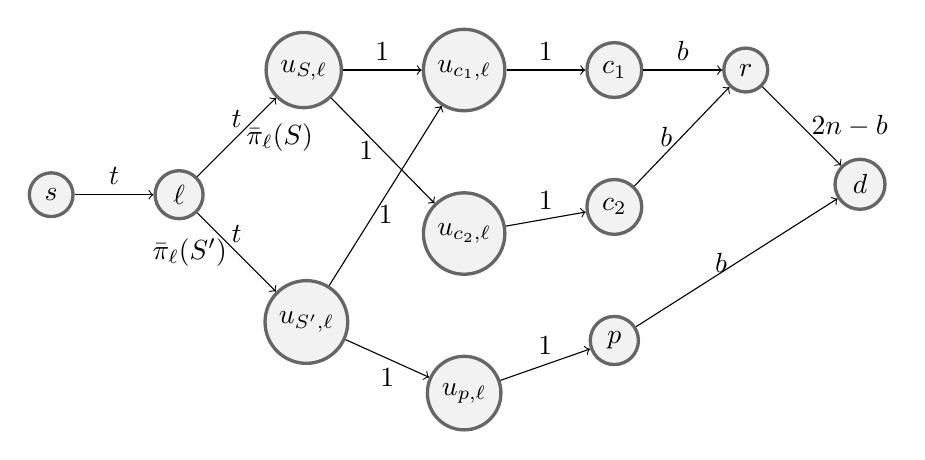
\begin{tikzpicture}[
mynode/.style={circle, draw=black!60, fill=black!5, very thick, minimum size=5mm},
]

\node[mynode](s){\normalsize $s$};
\node[mynode](ell)[right=of s]{\normalsize $\ell$};

\node[mynode](us1ell)[above right=of ell]{\normalsize  $u_{S,\ell}$};
\node[mynode](us2ell)[below right=of ell]{\normalsize $u_{S',\ell}$};

\node[mynode](uc1ell)[right=of us1ell]{\normalsize $u_{c_1,\ell}$};
\node[mynode](uc2ell)[below=of uc1ell]{\normalsize $u_{c_2,\ell}$};
\node[mynode](upell)[below=of uc2ell]{\normalsize $u_{p,\ell}$};

\node[mynode](c1)[right=of uc1ell]{\normalsize $c_1$};
\node[mynode](c2)[below=of c1]{\normalsize $c_2$};
\node[mynode](p)[below=of c2]{\normalsize $p$};

\node[mynode](r)[right=of c1]{\normalsize $r$};
\node[mynode](d)[below right=of r]{\normalsize $d$};


\draw[->](s) -- (ell) node [midway, above] {\normalsize $t$};

\draw[->](ell) -- (us1ell) node [midway, above] {\normalsize $t$} node [midway, right] {\normalsize $\bar{\pi}_{\ell}(S)$} ;
\draw[->](ell) -- (us2ell) node [midway, above] {\normalsize $t$} node [midway, left] {\normalsize $\bar{\pi}_{\ell}(S')$} ;

\draw[->](us1ell) -- (uc1ell) node [midway, above] {\normalsize $1$};
\draw[->](us1ell) -- (uc2ell) node [midway, left] {\normalsize $1$};
\draw[->](us2ell) -- (uc1ell) node [midway, below] {\normalsize $1$};
\draw[->](us2ell) -- (upell) node [midway, below] {\normalsize $1$};

\draw[->](uc1ell) -- (c1) node [midway, above] {\normalsize $1$};
\draw[->](uc2ell) -- (c2) node [midway, above] {\normalsize $1$};
\draw[->](upell) -- (p) node [midway, above] {\normalsize $1$};

\draw[->](c1) -- (r) node [midway, above] {\normalsize $b$};
\draw[->](c2) -- (r) node [midway, left] {\normalsize $b$};

\draw[->](r) -- (d) node [midway, right] {\normalsize $2n-b$};
\draw[->](p) -- (d) node [midway, left] {\normalsize $b$};
\end{tikzpicture}
}
\caption{A sub-graph of $G(b)$ for $2$-approval. Assume that $S=\set{c_1,c_2}$ and $S'=\set{c_1,p}$. Edge labels are their capacity. Where edges have a second label, it is their cost. All other edge costs are zero.}
\label{flowExample}
\end{figure}

For any set $S \in \binom{C}{t}$, we let $\bar{\pi}_{\ell}(S)=\max_{c \in S}v_\ell(c)-t$.
We can assume w.l.o.g.\ that we know the value $b$, the final score of $p$ in the optimal demotion strategy (since we can try all the possible values for $b$ and choose the one resulting in the cheapest final solution). 
We shall construct a priced flow network $G(b)$ in which units of flow represent awarded points, as follows. The vertex set  $U = \set{s,d,r} \cup N \cup U_1 \cup U_2 \cup C$ is comprised of the following `layers' (visualized in \cref{flowExample}). 
\begin{itemize}
    \item $N$ (resp.\ $C$) represents the voter set (resp.\ candidate set); a flow unit passing through a vertex $\ell \in N$ (resp.\ $c \in C$) represents a point awarded by $\ell$ (resp. awarded to $c$).
    \item $U_1 = \setgiven{u_{S,\ell} \given S \in \binom{C}{t}, \ell \in N}$; a flow unit passing through a vertex $u_{S,\ell} \in U_1$ represents a point awarded by $\ell$ to a candidate in $S$ (the choice of \emph{which candidate} will be immediately discussed).
    \item $U_2 = \setgiven{u_{c,\ell} \given c \in C, \ell \in N} \in U_2$; a flow unit passing through a vertex $u_{c,\ell}$ represents a point awarded by $\ell$ to the candidate $c$.
    % \item $C$ representing the candidate set; a flow unit passing through a vertex $c \in C$ represents a point awarded to $c$.
    \item $s$ and $d$ are the \emph{source} and \emph{destination} vertices. $r$ represents any candidate other than $p$.
\end{itemize}
The edge set $E=E_1 \cup E_2 \cup E_3 \cup E_4 \cup E_5 \cup E_6$ is comprised of the following, where $\gamma(u,v)$ is the capacity of an edge $(u,v)$ and  $a(u,v)$ is its cost.
\begin{itemize}
    \item $E_1=\setgiven{(s,\ell) \given \ell \in N}$ with all capacities equal to $t$, guarantees that each voter has at most $t$ points to distribute.
    \item $E_2= \setgiven{(\ell, u_{S,\ell})\given \ell \in N, S \in \binom{C}{t}}$ with capacities equal to $t$, will be discussed later.
    \item $E_3=\setgiven{(u_{S,\ell}, u_{c,\ell})\given \ell \in N, c \in S}$ with all capacities equal to $1$, guarantees that each candidate can receive at most one point from a subset he is a member of.
    \item $E_4= \setgiven{(u_{c,\ell},c) \given c \in C, \ell \in N}$ with all capacities equal to $1$, guarantees that each candidate can receive at most one point from a specific voter.
    \item $E_5= \setgiven{(c,r) \given c \in \Cmp}$, with all capacities equal to $b$ guarantees that each candidate will receive at most $b$ points (where $b$ will be $p$'s final score).
    \item $E_6= \set{(p,d),(r,d)}$, where $\gamma(p,d)=b$ and $\gamma(r,d)=tn-b$. By later setting the desired flow value to $tn$, these edges will be saturated, and $p$'s score will be exactly $b$. 
\end{itemize}
For each edge $(\ell, u_{S,\ell}) \in E_2$, we let $a(\ell, u_{S,\ell}) = \bar{\pi}_{\ell}(S)$. All other edge costs are $0$. Finally we let $G(b)=(U,E,\gamma,a)$. An example of a sub-graph of $G(b)$ is shown in \cref{flowExample}.

% We set a default capacity of 1 and a default price of 0 for all the edges unless otherwise specified.
% For each edge $(s,\ell) \in E_1$ we set $\gamma(s,\ell)=t$.
% For each edge $(\ell, u_{S,\ell}) \in E_2$, we let $a(\ell, u_{S,\ell}) = \bar{\pi}_{\ell}(S)$ and $\gamma(\ell, u_{S,\ell})=t$.
% % For each edge $e \in E_3 \cup E_4$ we let $\gamma(e)=1$, $a(e)=0$.
% For each edge $(c,r) \in E_5$ we let $\gamma(c,r)=b$.
% We let $\gamma(p,d)=b$ and $\gamma(r,d)=tn-b$. Finally we let $G(b)=(U,E,\gamma,a)$. 

The main procedure is the following. Given $b$, construct $G(b)$, and run a \CMCF{} algorithm on it with a desired flow value $tn$ \cite{edmonds1972theoretical}. If it failed to find such a flow then return a \emph{fail} status; otherwise, denote the resulting network flow as $f$. We shall modify $f$ to become another flow $f'$ as follows.
For each voter $\ell$, let $S'_{\ell} = \setgiven{c \given f(u_{c,\ell},c)=1}$. We will prove that $\abs{S'_{\ell}}=t$. We define $f'(\ell, u_{S'_{\ell},\ell})=t$, $f'(u_{S'_{\ell},\ell}, u_{c,\ell})=\indic_{S'_{\ell}}(c)$, $f'(\ell,u_{S,\ell})=0$ for all $S \neq S'_{\ell}$, and $f'(u_{S,\ell}, u_{c,\ell})=0$ for all $S \neq S'_{\ell}$. 
% Note that $f'$ does not change the flow of $(u_{c,\ell},c)$ and therefore it does not impact the total flow, meaning that the flow $f'=tn$ is maximal as well.
Based on $f'$, we compute the following demotion strategy $Q$:  perform the necessary demotions such that for each $\ell$, the candidates in $S'_{\ell}$ become the top $t$ candidates in $v_\ell$; this is done by demoting all candidates $c' \notin S'_{\ell}$ for which $v_\ell(c') < \max_{c \in S'_{\ell}} v_\ell(c)$ to the bottom of $v_\ell$. 

Our approximation algorithm, denoted $\mathcal{M}$, repeats the above procedure for each $b \in [n]$, and returns the strategy $Q$ having the minimum cost out of all strategies computed.

Let $Q^{\star}$ be the optimal demotion strategy. In the following lemmas, we will argue that the above algorithm returns a demotion strategy $Q$ for which $\pi(Q) \leq t\pi(Q^{\star})$.

% For any flow $f$, let $R^f_\ell=\setgiven{S \given  f(\ell, u_{S, \ell})\geq 1}$.
% \begin{lemma}
% Let $\set{S'_{\ell}}_{\ell \in N}$ be a collection of size-$t$ subsets of $C$. Then there exist a flow $f$ having cost $\af$ such that  $R^f_\ell = \set{S'_\ell}$ for each $\ell$ if and only if the exists a demotion strategy $Q$ having cost $\af/t$ such that for each $\ell$, the candidates in   $S'_\ell$ are the top-$t$ candidates in $v_\ell$ following the demotion operations.
% % For any flow $f$ such that $\abs{f} = tn$, let $R^f_\ell=\setgiven{S \given  f(\ell, u_{S, \ell})\geq 1}$. Then  $\abs{R^f_\ell}=1$ for each $\ell$ if and only if
% \end{lemma}
% \begin{proof}
% Let $f$ be a  flow satisfying the above properties, 
% % since $\abs{f} = tn$, and every voter $\ell$ has an incoming capacity of $t$, each voter transfers exactly $t$ flow units to candidates. Fix a voter $\ell$. Since $\gamma(u_{c,\ell},c) = 1$ for each $c$, there must be exactly $t$ candidates receiving a unit flow from $\ell$. 
% % If $\abs{R^f_\ell}=1$, then necassrily $R^f_\ell=\set{S'_\ell}$, where $S'_\ell$ is these $t$ candidates. A unique demotion strategy is obtain by having $\ell$ demote the 
% We define $Q$ such that 

% Starting with a demotion strategy $Q$, let let $R^f_\ell= \set{S'_\ell}$, where $S'_\ell$ is the top-$t$ candidates in $v_\ell$ following the demotion operations.  Now define $f$ as follows. $f(\ell, u_{S'_\ell,\ell}) = t, f(u_{S'_\ell,\ell}, u_{c,\ell}) = \mathbf{1}[c \in S'_\ell], f(u_{c,\ell},c) = \mathbf{1}[c \in S'_\ell], f(c,r) = s(c),f(r,d)=\sum_{c \in \Cmp}s(c)=tn-b^\star, f(p,d)=b^\star$. All other edges will have $0$ flow. It can be easily verified that all the flow conditions are satisfied, and that $\abs{f} = f(r,d)+f(p,d) = tn$.
% \end{proof}


% s proved in \cref{flowIsMaximal}, when $b = b^{\star}$ there exists a maximal flow $tn$ in $G(b^{\star})$ and therefore in this iteration our algorithm will find a flow $f'$ such that $\abs{f'} = tn$ and $\sum_{e \in E}a(e)f'(e) \leq t \sum_{e \in E}a(e)f_{\min}(e) \leq t \sum_{e \in E}a(e)f^\star(e)$, where $f_{\min}$ (resp.\  $f^\star$) is the min-cost flow (resp.\ flow induced by the optimal strategy as detailed in \Cref{flowIsMaximal}). Now notice that for any flow $f$,  $\af = \sum_{e \in E_2}a(e)f(e) = \sum_{\ell,S}a(\ell, u_{S, \ell})f(\ell, u_{S, \ell})$ 
% as all edges not in $E_2$ have zero cost. We obtain that $\pi(Q) = 
% \sum_{\ell \in N}a(\ell, u_{S'_\ell, \ell}) = \sum_{\ell \in N}a(\ell, u_{S'_\ell, \ell})f(\ell, u_{S'_\ell, \ell})/t \leq \sum_{\ell \in N}a(\ell, u_{S'_\ell, \ell})f^\star(\ell, u_{S'_\ell, \ell})=  t \sum_{\ell \in N}a(\ell, u_{S'_\ell, \ell})\leq t\pi(Q^\star)$ wher
\begin{lemma} \label{edgesCostsLemma}
For a size-$t$ set $S$, the minimal price for making all the candidate in $S$ become the top $t$ candidates in $v_\ell$ is $\bar{\pi}_{\ell}(S)=\max_{c \in S}v_\ell(c)-t$.
\end{lemma}
\begin{proof}
Let $c' = \argmax_{c \in S}v_\ell(c)$ be the bottom-most candidate in $S$ w.r.t.\ $v_{\ell}$. The number of candidates not in $S$ who are ranked before him in $v_\ell$ is exactly $v_\ell(c')-t$.
% Each demotion operation has a unit cost. In order to make all the candidates in $S_\ell$ first in $v_\ell$ we must demote all the candidates above any candidate of the set $S_\ell$ in $v_\ell$. Let $c_{max}= \argmax_{c \in S_\ell} v_\ell(c)$. There are $v_\ell(c_{max}) - 1$ candidates above him, but there are exactly $t-1$ candidates that are in $S_\ell$ and we do not want to demote them. In total we have $v_\ell(c_{max}) -t$ operations.
\end{proof}
Let $b^\star$ be the final score of $p$ under  $Q^\star$.
\begin{lemma}\label{flowIsMaximal}
There exists a potential flow $f^\star$ in $G(b^\star)$ where $\abs{f^\star} = tn$ and $\Aoper{f^\star} = t\cdot \pi(Q^\star)$.
\end{lemma}
\begin{proof}
 We define $f^\star$ in $G(b^\star)$ as follows. For each $\ell$, let $S^\star_\ell$ be the candidates $\ell$ approves of following the demotion operations in $Q^\star$, and let $s^\star(c)$ be the resulting score of $c$. Set $f^\star(\ell, u_{S^\star_\ell,\ell}) = t$, $f^\star(u_{S^\star_\ell,\ell}$, $u_{c,\ell}) = \indic_{S^\star_{\ell}}(c)$, $f^\star(u_{c,\ell},c) = \indic_{S^\star_{\ell}}(c)$, $f^\star(c,r) = s^\star(c)$, $f^\star(r,d)=\sum_{c \in \Cmp}s^\star(c)=tn-b^\star$,  $f(p,d)=b^\star$. All other edges will have $0$ flow. It can be easily verified that all the flow conditions are satisfied, that $\abs{f^\star} = f(r,d)+f(p,d) = tn$, and that $\Aoper{f^\star} =  \sum_{\ell}a(\ell, u_{S^\star_\ell, \ell})f^\star(\ell, u_{S^\star_\ell, \ell})= t \cdot \sum_{\ell}a(\ell, u_{S^\star_\ell, \ell}) =  t \cdot \sum_{\ell}\bar{\pi}_{\ell}(S^\star_\ell)= t\cdot \pi(Q^\star)$.
\end{proof}
The following lemmas assume that the algorithm did not fail on $G(b)$, and thus $\abs{f} = tn$.
\begin{lemma}
For each voter $\ell$, $\abs{S'_\ell}=t$. $f'$ is well-defined, is a valid flow, and  $\abs{f'} = tn$.
\end{lemma}
\begin{proof}
We have that $\abs{f} = tn$. As every voter $\ell$ has an incoming capacity of $t$, each voter transfers exactly $t$ flow units to candidates. 
Fix a voter $\ell$. Since $\gamma(u_{c,\ell},c) = 1$ for each $c$, there must be exactly $t$ candidates
such that each receives a unit flow from $\ell$. Therefore $\abs{S'_\ell}=t$ and $u_{S'_\ell, \ell}$ is a node in $G(b)$. When defining $f'$, after identifying the set $S'_\ell$, the algorithm simply reroutes the $t$ flow units to the the candidates in $S'_\ell$ through $u_{S'_\ell, \ell}$, thus the flow value is maintained.
% The flow value is $tn$ units. As every voter $\ell$ has an incoming capacity of $t$ and as $\gamma(u_{c,\ell},c) = 1$ for each $\ell,c$, the only way to reach the resulting flow is by having, for each $\ell$, exactly $t$ edges $(u_{c,\ell},c)$ s.t.\ $f(u_{c,\ell},c)=1$.
% ($f(s,\ell)=t$). As the only option of flowing from the node $\ell$ to $d$ is through the edges $(u_{c,\ell}, c)$ and $\gamma(u_{c,\ell}, c)=1$, this means we have $t$ different edges $(u_{c,\ell},c)$ s.t. $f(u_{c,\ell},c)=1$. In conclusion, $\abs{S'_\ell}=t$.
\end{proof}

\begin{lemma} \label{totalPriceLemma}
It holds that $\Aoper{f'} \leq t \cdot \Aoper{f}$.
\end{lemma}
\begin{proof}
Fix a voter $\ell$, and let $R=\setgiven{S \given  f(\ell, u_{S, \ell})\geq 1}$. Now consider the candidate set $C' = \bigcup_{S \in R}S$ and the set $S_{\max}=\argmax_{S\in R} \bar{\pi}_{\ell}(S)$. Let $c'$ be the candidate $c \in C'$ maximizing $v_\ell(c)$ and notice that $c' \in S_{\max}$. Now consider $S'_{\ell}$ as defined by the algorithm and notice that $S'_{\ell} \subseteq C'$ by the flow properties: a unit of flow which reaches a candidate $c$ from $\ell$ must pass through some node $u_{S,\ell}$ such that $c \in S$. Therefore---applying \Cref{edgesCostsLemma}---$\bar{\pi}_{\ell}(S') \leq \bar{\pi}_{\ell}(S_{\max})$.

It follows that $a(\ell, u_{S'_\ell, \ell})f'(\ell, u_{S'_\ell, \ell}) =t \cdot a(\ell, u_{S'_\ell, \ell})  \leq t\cdot  a(\ell, u_{S_{\max}, \ell}) \leq 
t\cdot \sum_{S \in R}a(\ell, u_{S, \ell}) f(\ell, u_{S, \ell})$.
% , where the last inequality follows from the fact that $\sum_{S \in R}f(\ell, u_{S, \ell}) = t$ (otherwise reaching a flow value of $tn$ is impossible). 
The lemma follows by summing the last inequality over all voters $\ell \in N$, and recalling that for each edge $e \notin E_2$, $a(e)=0$.
% ---------------------------------
% let $S_{\max}=\arg\max_{S} \setgiven{\bar{\pi}(S) \given f(u_{S,\ell}, u_{c'_\ell,\ell})=1}$. Now let $c'$ be the candidate maximizing $v_\ell(c')$ in $S'_\ell$,  and likewise, let  $c''$ be the candidate maximizing $v_\ell(c'')$ in $S_{\max}$. Notice that $c''$ is in particular the candidate maximizing $v_\ell(c'')$ in $\bigcup_{S \in \setgiven{\bar{\pi}(S) \given f(u_{S,\ell}, u_{c'_\ell,\ell})=1}}S$
% $v_\ell(c') \leq v_\ell(c'')$,
% let $c'_\ell=\argmax_{c \in S'_\ell} v_\ell(c)$ the bottom-most candidate that was promoted to the top-most  $t$ candidates in $v_\ell$. 
% by both $f$ and $f'$ as they both choose the same candidates). Let $S_{max}$ be the set s.t. $f(u_{S,\ell}, u_{c'_\ell,\ell})=1$ (there must be exactly one set holding this property since $f(u_{c'_\ell,\ell},c'_\ell)=1$). Let $a^{\star}_\ell = a(\ell,u_{S_{max},\ell})$. It holds that $a^{\star}_\ell = v_\ell(c'_\ell)-t$ from the definition of $c'_\ell$ and from \cref{edgesCostsLemma}.
% Also, for every edge $(\ell,u_{S,\ell})$ s.t. $f(\ell,u_{S,\ell}) > 0$, $a(\ell,u_{S,\ell}) \leq v_\ell(c'_\ell)-t = a^{\star}_\ell$ (because all the other promoted candidates have a smaller cost than $c'_\ell$), so $a(\ell,u_{S'_\ell, \ell}) \leq a^{\star}_\ell$
% In conclusion, the total price $a(f) \geq \sum_\ell a^{\star}_\ell$. From the construction of $f'$, it holds that $a(f') \leq t\sum_\ell a^{\star}_\ell$ (because $f'(\ell, u_{S'_\ell, \ell})=t$). $a(f') \leq t a(f)$.
\end{proof}

\begin{theorem}
Algorithm $\mathcal{M}$ returns a valid solution $Q$ making $p$ win, and $\pi(Q) \leq t \pi(Q^{\star})$.
\end{theorem}
\begin{proof}
It is enough to show that in the iteration where $b = b^{\star}$, we find a solution  $Q' $ such that $\pi(Q' ) \leq t \pi(Q^{\star})$.

As proven in \Cref{flowIsMaximal}, when $b = b^{\star}$ there exists a maximal flow $tn$ in $G(b^{\star})$ and therefore our algorithm will find such a flow. Consider $f$ and $f'$, the min-cost flow and the constructed flow in this iteration. Also consider  $f^\star$, the flow induced by the optimal strategy as detailed in \Cref{flowIsMaximal}.

It holds that $\abs{f'} = tn$ and $\Aoper{f'} \leq t \cdot \Aoper{f} \leq t \cdot \Aoper{f^\star} $. Since $\abs{f'} = tn$, then $f'(p,d)=b$. Since $f'(c,r)\leq b$ for all $c \in \Cmp$, $p$ is necessarily winning.

For the flow $f'$,  it holds that 
\begin{align*}
    \Aoper{f'} &= \sum_{\ell \in N}a(\ell, u_{S'_\ell, \ell})f'(\ell, u_{S'_\ell, \ell})\\
    &= t \cdot \sum_{\ell \in N}a(\ell, u_{S'_\ell, \ell})\\
    &=  t \cdot \sum_{\ell \in N}\bar{\pi}_{\ell}(S'_\ell)\\
    &= t\cdot \pi(Q')\ .
\end{align*}
We obtain that $\pi(Q') = \Aoper{f'}/t \leq  \Aoper{f^\star} = t \cdot \pi(Q^\star)$, where the inequality follows from \Cref{totalPriceLemma} and the final equality from \Cref{flowIsMaximal}.
% after the demoting operations of $Q^{\star}$, there exists a maximal flow to $G(b^{\star})$ of $tn$. With the flows $f$ and $f'$ of our algorithm for only $G(b^{\star})$, it holds that $a(f) \leq t \pi(Q^{\star})$ because we can solve the flow network by computing the set $S_\ell$ of the top $t$ candidates of $v_\ell$ after the demoting operation of $Q^{\star}$ for every $\ell$, and flow $t$ units $f^{\star}(\ell, u_{S_\ell, \ell})=t$. There exists a solution with the above flow $f^{\star}$ (because $p$ wins after $Q^{\star}$), and therefore $a(f) \leq a(f^{\star})$. Because the price $a(f^{\star})$ is given by summing on all the voters the flow of $t$ units in $(\ell, u_{S_\ell, \ell})$ resulting on $t$ times the price of $a(\ell, u_{S_\ell, \ell})$ which is the minimal price of making the candidates in $S_\ell$ in the $t$ top ranks of $v_\ell$ (\cref{edgesCostsLemma}).In total $a(f) \leq a(f^{\star}) = t \pi(Q^{\star})$. In the same way, $a(f') = t \pi(Q_{b^{\star}})$ (because $Q_{b^{\star}}$ was extracted by $f'$). At last, by \cref{totalPriceLemma}, $\pi(Q) \leq \pi(Q_{b^{\star}}) = \dfrac{a(f')}{t} \leq a(f) \leq t \pi(Q^{\star})$.
\end{proof}
We make two important remarks: (a) our algorithm can be easily extended to support prices that are a function of the voters (by re-defining $a(\ell, u_{S,\ell})$ to be also multiplied by the voter's price); and (b) our algorithm provides an exact solution in the specific case of Plurality (as $t=1$).

\section{Borda}
In this section we will show $\NP$-hardness and a $3$-multiplicative approximation for Borda.
\subsection{\boldmath{$\NP$}-Hardness}\label{sec:borda_hardness}
\begin{theorem}\label{thr:borda_hardness}
Given a value $k$, determining whether there exists a solution to Borda-\SB{} with at most $k$ demotions  is $\NP$-hard.
\end{theorem}
\begin{proof}
Given an instance $I=(U,\mathcal{S})$ of \SC{} and a desired cover size $k \leq \bar{m}$, we define a reduction as follows. 

We define the candidate set $C=U \cup  D \cup \set{p,a,b}$, where $D=\set{d_0,\ldots,d_{\bar{n}-2}}$ is a set of $\bar{n}-1$ dummy candidates, $p$ is the preferred candidate and $a,b$ are  two additional candidates. We let $D_{<q}=\set{d_0,\ldots,d_{q-1}}$ and $D_{\geq q}=\set{d_{q},\ldots,d_{\bar{n}-2}}$. 

The preference profile is defined as follows. For each set $S_i \in \mathcal{S}$, we define two preference orders $v_i^1,v_i^2$, such that
\begin{align}
    v_i^1 &= \ora{D_{\geq \abs{S_i}}} \succ  \ora{S_i}  \succ  a \succ b \succ \ora{U \setminus S_i}\succ \ora{D_{<\abs{S_i}}} \succ p   \\
    v_i^2 &=  p  \succ \ola{D_{<\abs{S_i}}} \succ \ola{U \setminus S_i} \succ b \succ a \succ \ola{S_i} \succ  \ola{D_{\geq \abs{S_i}}}\ . 
\end{align}
In addition, we define the following two preference orders:
\begin{align}
    \bar{v} &=  \ora{D} \succ a \succ b \succ  \ora{U}  \succ p \\
    \hat{v} &=  p \succ \ola{U}  \succ a \succ b \succ \ola{D} \ . 
\end{align}
Finally, we define the following two preference orders:
\begin{align}
    \bar{v}' &= \ora{D} \succ a \succ \ora{U} \succ b  \succ p  \\
    \hat{v}' &=  p \succ \ola{U}  \succ a \succ b \succ \ola{D}\ . 
\end{align}
We let 
$$V=\set{v_i^1,v_i^2}_{i=1}^{\bar{m}} \cup \set{\bar{v}_j, \hat{v}_j}_{j=1}^{k(\bar{n}+3)-1} \cup \set{\bar{v}', \hat{v}'}\ ,$$ 
where each $\bar{v}_j$ (resp.\  $\hat{v}_j$) is a copy of $\bar{v}$ (resp.\  $\hat{v}$).\footnote{While $V$ is a list of preference orders, with a slight abuse of notation, we have defined it using set operations.} Let $E = (C,V)$ be the resulting election. 
\begin{lemma}
% Let $s(u_1)=x$. 
For $E$, it holds that  $\diff(a,p)=k(\bar{n}+3)$,  that $\diff(p,b)= k(\bar{n}+3) + \bar{n}$, and that
  $\diff(p,d)= 0$  for every $d \in D$. In addition, $\diff(u_1,p)=\cdots=\diff(u_{\bar{n}},p)=1$.
\end{lemma}
By summing the points awarded to each candidate. To see that more easily, notice that each pair of preference orders defined above awards $m-1$ points to each candidate, unless the following event occurs: whenever $c \succ c'$ in \emph{both} of the pair's preference orders, it effectively means that a points is `transferred' from $c'$ to $c$.
% JOURNAL
% \begin{proof}
% Assume that we start with an empty preference profile, first add the votes $\set{v_i^1,v_i^2}_{i=1}^{\bar{m}}$, then the votes $\set{\bar{v}_j, \hat{v}_j}_{j=1}^{k(\bar{n}+3)-2}$ and finally $\set{\bar{v}', \hat{v}'}$.

% When the preference profile is empty, obviously $\diff(c,c')=0$ for every $c,c' \in C$. 
% Adding $\set{v_i^1,v_i^2}_{i=1}^{\bar{m}}$ preserves these relative scores as $v_i^1$ and  $v_i^2$ are the same preference order, only that one is reversed w.r.t.\ the other. Therefore, $\diff(c,c')$ is still $0$ for every $c,c' \in C$.

% Each pair of votes in $\set{\bar{v}_j, \hat{v}_j}_{j=1}^{k(\bar{n}+3)-1}$ adds an additional point to $a$ on the expense of $b$---as $a \succ b$ in \emph{both}  $\bar{v}$  and $\hat{v}$---while preserving the relative scores of all other candidates. Thus  $\diff(c,c')=0$ for every $c,c' \notin \set{a,b}$, but $\diff(a,c) = k(\bar{n}+3)-2$ if $c \neq b$ and $\diff(b,c) = -k(\bar{n}+3)+2$ if $c \neq a$. Obviously, $\diff(a,b) = 2k(\bar{n}+3)-4$.

% Finally, the last pair $\set{\bar{v}', \hat{v}'}$ adds a point to each of $\set{a} \cup U$ on the expends of $b$.
% \end{proof}

\begin{lemma}\label{lem:pushed}
Let $Q$ be a winning demotion strategy for $E$ with $k$ demotion operations. Then all bribed voters have votes of types $v_i^1$, $\bar{v}$, or $\bar{v}'$, and in each of them  $a$ was demoted by $\bar{n}+2$ positions.
\end{lemma}
\begin{proof}
% TODO(orgad): s(p) is not defined (this is supposed to mean "the final score of p" - after the campaign).
Let $s(c)$ be the score of candidate $c$ after the demotion operations.
Since we have $k$ demotion operations, $s(p)$ will be at most $\sigma(p)+k$. To make $p$ indeed win we require that $s(a) \leq s(p)$, thus $a$ should lose \emph{at least} $k(\bar{n}+2)$ points. However, notice that for each voter, $a$ can be pushed down at most $\bar{n}+2$ positions. Indeed, only for voters of types $v_i^1, \bar{v}, \bar{v}'$, $a$ can be demoted by $\bar{n}+2$ positions (for all other voters, $a$ can be demoted by at most $\bar{n}+1$ positions). Thus, to reach the desired decrease in score, only voters of types $v_i^1, \bar{v}, \bar{v}'$ can be bribed, each once, and in each operation  $a$ will be demoted exactly $\bar{n}+2$ positions. As a result, $s(a)=s(p)=\sigma(p)+k$.
    % Now assume by contradiction that a voter of type $\hat{v}$ or  $\hat{v}'$ was bribed. Since $a$ was necessarily pushed down $n+2$ positions, all candidates in $D_q \cup \set{p,b}$ received each a point and as such, $\diff(p,u)$ has not changed for each $u \in U$ by bribing this voter. However, since $p$ now wins, for each $u$ it holds that $s'(p) \geq s'(u)$.
    \end{proof}
We are now ready to complete the proof of \Cref{thr:borda_hardness} by showing that
$E$ has a winning strategy with $k$ operations if and only if $U$ can be covered by $k$ subsets of $\mathcal{S}$.

\textit{Completeness:} Let $\mathcal{S}'$ be a valid $k$-cover. For each $S_i \in \mathcal{S}'$, bribe $v_i^1$ and move $a$ to the last position in $v_\ell$. Notice that now $s(p) =s(a) = \sigma(p)+k$. Now focus on the effect of bribing a single voter $v_i^1$:  it does not change the value $\diff(p,u)$ for each $u \in U\setminus S_i$, but increases $\diff(p,u)$ by $1$ for each $u \in S_i$. Since $\mathcal{S}'$  is a proper cover, it means that according to our scheme, for each $u$ there exists at least one bribed voter $v_i^1$  who  increases $\diff(p,u)$ by $1$ (this is a voter $v_i^1$ for which $S_i \in \mathcal{S}'$ and $u \in S_i$), thus at the end of the bribery process, $\diff(p,u) \geq 0$. We have just showed that $s(p) \geq s(u)$ for each $u \in U$, and that $s(p) \geq s(a)$. As for the remaining candidates in $D \cup \set{b}$, notice that at first they were ranked equally or less than $p$, and that each time one of them was promoted, $p$ was promoted as well, and therefore $\diff(p,c)$ does not decrease for each $c \in D \cup \set{b}$. We conclude that as a result of this bribery scheme, $p$ now wins.

\textit{Soundness:} Assume that $p$ can be made to win by bribing $k$ voters, and consider the corresponding demotion strategy. By \Cref{lem:pushed}, in all bribed votes  $a$ was pushed down $\bar{n}+2$ positions. Now observe only the bribed voters of type $v_i^1$. Since  for each $u \in U$ it held before that $\diff(p, u) = -1$, but now $\diff(p, u) \geq 0$, we bribed at least one voter $v_i^1$ such that $u \in S_i$, which allowed $\diff(p, u)$ to increase by a point. Therefore, the collection $\mathcal{S}' = \setgiven{S_i \in \mathcal{S} \given v_i^1 \text{ is bribed}}$ constitutes a valid cover. Since $\abs{\mathcal{S}'} \leq k$ 
% (and if $\abs{\mathcal{S}'} < k$, we can arbitrarily add subsets for $\mathcal{S}$ to the cover until $\abs{\mathcal{S}'} = k$), 
we are done.
\end{proof}



% For brevity, the proof is deferred to the appendix. We do detail its main idea here. Given an instance $I=(U,\mathcal{S})$ of \SC{} and a desired cover size $k \leq \bar{m}$, we reduce it to Borda-\SB{}. This is done by defining the candidate set $C=U \cup  D \cup \set{p,a,b}$, where $D=\set{d_0,\ldots,d_{\bar{n}-2}}$ is a set of $\bar{n}-1$ dummy candidates, $p$ is the preferred candidate and $a,b$ are  two additional candidates. We let $D_{<q}=\set{d_0,\ldots,d_{q-1}}$ and $D_{\geq q}=\set{d_{q},\ldots,d_{\bar{n}-2}}$. The preference profile includes, for each set $S_i \in \mathcal{S}$, a preference order
% \begin{equation*}
%     v_i^1 = \ora{D_{\geq \abs{S_i}}} \succ  \ora{S_i}  \succ  a \succ b \succ \ora{U \setminus S_i}\succ \ora{D_{<\abs{S_i}}} \succ p\ .   
% \end{equation*}
% There are several other votes in the preference profile, which are used to create a scenario where the \emph{only} way to make $p$ win, is by demoting $a$ to be last for each vote $v_i^1$ such that $S_i$ is part of the set cover. Such operation decreases the score difference between any candidate in $S_i$ and $p$ by exactly $1$. 

% \iffalse{
% \begin{proof}
% Given an instance $I=(U,\mathcal{S})$ of \SC{} and a desired cover size $k \leq \bar{m}$, we build the reduction as follows. 

% We define the candidate set $C=U \cup  D \cup \set{p,a,b}$, where $D=\set{d_0,\ldots,d_{\bar{n}-2}}$ is a set of $\bar{n}-1$ dummy candidates, $p$ is the preferred candidate and $a,b$ are  two additional candidates. We let $D_{<q}=\set{d_0,\ldots,d_{q-1}}$ and $D_{\geq q}=\set{d_{q},\ldots,d_{\bar{n}-2}}$. 

% The preference profile is defined as follows. For each set $S_i \in \mathcal{S}$, we define two preference orders $v_i^1,v_i^2$, such that
% \begin{align}
%     v_i^1 &= \ora{D_{\geq \abs{S_i}}} \succ  \ora{S_i}  \succ  a \succ b \succ \ora{U \setminus S_i}\succ \ora{D_{<\abs{S_i}}} \succ p   \\
%     v_i^2 &=  p  \succ \ola{D_{<\abs{S_i}}} \succ \ola{U \setminus S_i} \succ b \succ a \succ \ola{S_i} \succ  \ola{D_{\geq \abs{S_i}}}\ . 
% \end{align}
% In addition, we define the following two preference orders:
% \begin{align}
%     \bar{v} &=  \ora{D} \succ a \succ b \succ  \ora{U}  \succ p \\
%     \hat{v} &=  p \succ \ola{U}  \succ a \succ b \succ \ola{D} \ . 
% \end{align}
% Finally, we define the following two preference orders:
% \begin{align}
%     \bar{v}' &= \ora{D} \succ a \succ \ora{U} \succ b  \succ p  \\
%     \hat{v}' &=  p \succ \ola{U}  \succ a \succ b \succ \ola{D}\ . 
% \end{align}
% We let 
% $$V=\set{v_i^1,v_i^2}_{i=1}^{\bar{m}} \cup \set{\bar{v}_j, \hat{v}_j}_{j=1}^{k(\bar{n}+3)-1} \cup \set{\bar{v}', \hat{v}'}\ ,$$ 
% where each $\bar{v}_j$ (resp.\  $\hat{v}_j$) is a copy of $\bar{v}$ (resp.\  $\hat{v}$).\footnote{While $V$ is a list of preference orders, with a slight abuse of notation, we have defined it using set operations.}

% We denote the above reduction procedure as $f$, and let $E = (C,V) = f(I,k)$. 

% \begin{lemma}
% % Let $s(u_1)=x$. 
% In $f(I,k)$, it holds that  $\diff(a,p)=k(\bar{n}+3)$,  that $\diff(p,b)= k(\bar{n}+3) + \bar{n}$, and that
%   $\diff(p,d)= 0$  for every $d \in D$. In addition, $\diff(u_1,p)=\cdots=\diff(u_{\bar{n}},p)=1$.
% \end{lemma}
% Proof omitted, as it is based on summing awarded points.
% % JOURNAL
% % \begin{proof}
% % Assume that we start with an empty preference profile, first add the votes $\set{v_i^1,v_i^2}_{i=1}^{\bar{m}}$, then the votes $\set{\bar{v}_j, \hat{v}_j}_{j=1}^{k(\bar{n}+3)-2}$ and finally $\set{\bar{v}', \hat{v}'}$.

% % When the preference profile is empty, obviously $\diff(c,c')=0$ for every $c,c' \in C$. 
% % Adding $\set{v_i^1,v_i^2}_{i=1}^{\bar{m}}$ preserves these relative scores as $v_i^1$ and  $v_i^2$ are the same preference order, only that one is reversed w.r.t.\ the other. Therefore, $\diff(c,c')$ is still $0$ for every $c,c' \in C$.

% % Each pair of votes in $\set{\bar{v}_j, \hat{v}_j}_{j=1}^{k(\bar{n}+3)-1}$ adds an additional point to $a$ on the expense of $b$---as $a \succ b$ in \emph{both}  $\bar{v}$  and $\hat{v}$---while preserving the relative scores of all other candidates. Thus  $\diff(c,c')=0$ for every $c,c' \notin \set{a,b}$, but $\diff(a,c) = k(\bar{n}+3)-2$ if $c \neq b$ and $\diff(b,c) = -k(\bar{n}+3)+2$ if $c \neq a$. Obviously, $\diff(a,b) = 2k(\bar{n}+3)-4$.

% % Finally, the last pair $\set{\bar{v}', \hat{v}'}$ adds a point to each of $\set{a} \cup U$ on the expends of $b$.
% % \end{proof}

% \begin{lemma}\label{lem:pushed}
% Let $Q$ be a winning demotion strategy for $f(I,k)=E$ with $k$ demotion operations. Then all bribed voters have votes of types $v_i^1$, $\bar{v}$, or $\bar{v}'$, and in each of them  $a$ was demoted by $\bar{n}+2$ positions.
% \end{lemma}
% \begin{proof}
%  Since we have $k$ demotion operations, $p$'s final score will be at most $s'(p) = \sigma(p)+k$. To make $p$ indeed win we require that $s'(a) \leq s'(p)$, thus $a$ should lose at least $k(\bar{n}+2)$ points. However, notice that for each voter, $a$ can be pushed down at most $\bar{n}+2$ positions. Indeed, only for voters of types $v_i^1, \bar{v}, \bar{v}'$, $a$ can be demoted by $\bar{n}+2$ positions (for all other voters, $a$ can be demoted by at most $\bar{n}+1$ positions). Thus, to reach the desired decrease in score, only voters of types $v_i^1, \bar{v}, \bar{v}'$ can be bribed, each once, and in each operation  $a$ will be demoted exactly $\bar{n}+2$ positions.
%     % Now assume by contradiction that a voter of type $\hat{v}$ or  $\hat{v}'$ was bribed. Since $a$ was necessarily pushed down $n+2$ positions, all candidates in $D_q \cup \set{p,b}$ received each a point and as such, $\diff(p,u)$ has not changed for each $u \in U$ by bribing this voter. However, since $p$ now wins, for each $u$ it holds that $s'(p) \geq s'(u)$.
%     \end{proof}
% We are now ready to complete the proof of Theorem \ref{thr:borda_hardness}. That is, we show that
% $f(I,k)$ has a winning demotion strategy with $k$ operations if and only if $U$ can be covered by $k$ subsets of $\mathcal{S}$.

% \textit{Completeness:} Let $\mathcal{S}'$ be a valid $k$-cover. For each $S_i \in \mathcal{S}'$, bribe $v_i^1$ and move $a$ to the last position in $v_\ell$. Notice that now $s'(p) =s'(a) = \sigma(p)+k$. Now focus on the effect of bribing a single voter $v_i^1$:  it does not change the value $\diff(p,u)$ for each $u \in U\setminus S_i$, but increases $\diff(p,u)$ by $1$ for each $u \in S_i$. Since $\mathcal{S}'$  is a proper cover, it means that according to our scheme, for each $u$ there exists at least one bribed voter $v_i^1$  who  increases $\diff(p,u)$ by $1$ (this is a voter $v_i^1$ for which $S_i \in \mathcal{S}'$ and $u \in S_i$), thus at the end of the bribery process, $\diff(p,u) \geq 0$. We have just showed that $s'(p) \geq s'(u)$ for each $u \in U$, and that $s'(p) \geq s'(a)$. As for the remaining candidates in $D \cup \set{b}$, notice that at first they were ranked equally or less than $p$, and that each time one of them was promoted, $p$ was promoted as well, and therefore $\diff(p,c)$ remains unchanged for each $c \in D \cup \set{b}$. We conclude that as a result of this bribery scheme, $p$ now wins.

% \textit{Soundness:} Assume that $p$ can be made to win by bribing $k$ voters, and consider the corresponding demotion strategy. By \Cref{lem:pushed}, in all bribed votes  $a$ was pushed down $\bar{n}+2$ positions. Now observe only the bribed voters of type $v_i^1$. Since  for each $u \in U$ it held before that $\diff(p, u) = -1$, but now $\diff(p, u) \geq 0$, we bribed at least one voter $v_i^1$ such that $u \in S_i$, which allowed $\diff(p, u)$ to increase by a point. Therefore, the collection $\mathcal{S}' = \setgiven{S_i \in \mathcal{S} \given v_i^1 \text{ is bribed}}$ constitutes a valid cover. Since $\abs{\mathcal{S}'} \leq k$ 
% % (and if $\abs{\mathcal{S}'} < k$, we can arbitrarily add subsets for $\mathcal{S}$ to the cover until $\abs{\mathcal{S}'} = k$), 
% we are done.
% \end{proof}
% }\fi

\subsection{Approximation}
% We will show an approximation of factor 3 for \SB{} with Borda scoring rule, when $\delta=m$ meaning we can choose how many places a voter will move down a specific targeted candidatate, and a voter can be targeted multiple times ($\beta=\infty$). We will denote this model as \CUBNBwTA.
The main idea behind our approximation is noticing that the hardness of \SB{} under Borda stems from the fact that when we demote a candidate by $\delta$ positions, then $\delta$ candidates receive a point. Now assume that we ignore this issue for a moment. This is equivalent to  range voting (RV) where each voter awards a score between $0$ and $m-1$ to each candidate. Here, demoting a candidate---e.g., by having a voter decrease her awarded score by $\delta$ points---does not have any consequence on the score of other candidates.

\begin{algorithm}[tb]
\caption{$\CF((C,\bar{V}), k, T)$ \label{ConsequenceFreeAlg}}
\SetKwInOut{Input}{input}
\SetKw{Break}{break}
\SetKw{Fail}{fail}
$Q \gets \varnothing$\;
\ForEach{$c \in C$}{
$S_{c} \gets \setgiven{ (\ell, \delta) \given (c, \delta) \in \bar{v}_{\ell},\ \ell=1,\ldots,n }$\;
$s_c \gets \sigma(c)$\;
}
% \ForEach{$c \in C'$}{$\heap_{c} \gets \heapify(\setgiven{ (\ell, m- \bar{v}_{\ell}(c)) \given \ell \in N })$\;
% $s_c \gets \sigma(c)$}
\For{$i\gets 1$ \KwTo $k$}{
$C' \gets \setgiven{c \in C \given s_c > T}$\;
\If{$C' = \varnothing$}{\Break}
Pick an arbitrary  $c \in C'$.\;
 $(\ell',\delta') \gets \argmax_{(\ell,\delta) \in S_c}\delta$\;
% $\ell' \gets \argmin_{\ell} \bar{v}_{\ell}(c)$\;
% $\delta \gets m- \bar{v}_{\ell'}(c)$\;
% $(\ell, \delta) \gets \mathsf{extract\_max}(\heap_c)$\;
$Q \gets Q \cup \set{(\ell', c, \delta')}$\;
$S_{c} \gets S_{c} \setminus \set{(\ell',\delta') } $\;
$s_c \gets s_c - \delta'$\;
}
$C' \gets \setgiven{c \in C \given s_c > T}$\;
\leIf{$C' = \varnothing$}{\Return $Q$\label{ConsequenceFreeAlg:returnB}
}{\Fail}
\end{algorithm}

We  start by reducing our instance into a corresponding RV instance $\bar{E}$: we naturally translate a ranking in the $j$-th place of a candidate by a voter to awarding him a score of $\alpha_j=m-j$ by the voter. 
In the reduced instance, we look for the smallest $k$ for which we can make sure---using at most $k$ demotion operations---that all candidate scores do not exceed a bound $T = \sigma(p) + k$. We refer to \SB{} under RV with this goal as \emph{bounded} \SB{} under RV.
We denote the function that---given a RV instance, and the values $k$ and $T$---either returns a sequence of at most $k$ demotion operations or fails---as $\CF(\bar{E}, k, T)$. 


%In \Cref{ConsequenceFreeAlg} 
Computing $\CF{}$ is easily achievable by a greedy algorithm which iteratively: (a)  identifies a \emph{violating candidate} for which the score exceeds $T$; (b) finds the voter who awards him the maximal number of points; and (c) performs a demotion operation, decreasing the score given by this voter to the candidate to $0$. The algorithm for $\CF$ is illustrated as \Cref{ConsequenceFreeAlg}.

After finding the smallest $k$ for which $\CF(\bar{E}, k, \sigma(p) + k)$ succeeds, we take the resulting demotion strategy and apply it on the original Borda instance. Unfortunately, these operations now do have their consequences, and candidate scores might increase as a result of the demotion operations. However, we will prove that not by too much. In any case, $p$ might be losing. We address this by repeating the following procedure: we  find a voter who currently has $p$ at any position but the top one, and then swap $p$ and the candidate ranked above him by this voter. We shall repeat this step until $p$ is winning. The overall algorithm is described in \Cref{3k-approxAlg}.

% To do that, we will induce a new function $iso(V, C, t)$ (the voting profiles $V$ and the candidates $C$), and $\delta$ is a positive integer. $iso(V, C, t)$ computation is as follows:

% \iffalse
% \begin{algorithm}[tb]
% \caption{$\CF((C,\bar{V}), k, T)$ \label{ConsequenceFreeAlg}}
% \SetKwInOut{Input}{input}
% \SetKw{Break}{break}
% \SetKw{Fail}{fail}
% Let $C'= \setgiven{c \in C \given \sigma(c) > T}$\label{ConsequenceFreeAlg:C'}\;
% Let $Q=\varnothing$\;
% \ForEach{$c \in C'$}{$\heap_{c} \gets \heapify(\setgiven{ (\ell, \bar{v}_{\ell}(c)) \given \ell \in N })$\;
% $s_c \gets \sigma(c)$}
% \For{$i\gets 1$ \KwTo $k$}{
% $C'' \gets \setgiven{c \in C \given s_c > T}$\;
% \If{$C''$ is empty}{\Break}
% Pick an arbitrary  $c \in C''$.\;
% $(\ell, t) \gets \mathsf{extract\_max}(\heap_c)$\;
% $Q \gets Q \cup \set{(\ell, c, \delta)}$\;
% $s_c \gets s_c - \delta$\;
% }
% $C'' \gets \setgiven{c \in C \given s_c > T}$\;
% \leIf{$C''$ is empty}{\Return $Q$\label{ConsequenceFreeAlg:returnB}
% }{\Fail}
% \end{algorithm}
% \fi

\begin{algorithm}[tb]
\caption{\SB{} for Borda}
\label{3k-approxAlg}
\SetKwInOut{Input}{input}
\SetKw{Break}{break}
\SetKw{Continue}{continue}
\SetKw{Fail}{fail}
% \Input{An election $E=(C,V)$}
$\bar{V}=( \bar{v}_{\ell})_{\ell}$ where $\bar{v}_{\ell} = \setgiven{(c, \alpha_{v_\ell(c)})\given c \in C \setminus \set{p}}$\;
Let $\bar{E} = (C \setminus \set{p}, \bar{V})$\label{line:construct}\;
Let $k'$ be the minimum $k$ for which $\CF(\bar{E}, k, \sigma(p)+k)$ does not fail\label{3k-approxAlg:t-definition}\;
$Q \gets \CF(\bar{E}, k', \sigma(p)+k')$ \label{3k-approxAlg:BeforeBribe}\;
\ForEach{$(\ell, c, \delta) \in Q$ \label{3k-approxAlg:ConFreeBribes}}{
Demote $c$ in $v_{\ell}$ by $\delta$ positions.\;
}
\While{$p$ is not winning \label{3k-approxAlg:ReparePLoop}}{
Let $\ell \in N, c \in C \setminus \set{p}$  such that $c$ is ranked immediately before $p$ in $v_{\ell}$.\;
Demote $c$ in $v_{\ell}$ by one position.
}
\Return the sequence of demotion operations performed.\;
\end{algorithm}

% \begin{enumerate}
%     % \item $iso(V, C, t)$
%     \item $C' := \set{c \in C : u(c) > u(p) + t}$
%     \item if $|\var{C'}| > \var{t}$
%     \begin{enumerate}
%         \item return \emph{Failed}
%     \end{enumerate}
%     \item output = []
%     \item for $c \in C'$ do
%     \begin{enumerate}
%         \item while $u(c) > u(p) + t$
%         \begin{enumerate}
%             \item v = voter in which c has the highest score.
%             \item output.append((v, c))
%             \item Bribe($(v, c,m-v(c))$) (i.e., make c go down to the bottom in v's ranking)
%             % \item u(c) -= Borda(v(c)) (The borda score of c in v's voting).
%         \end{enumerate}
%     \item if $|output| > t$
%         \begin{enumerate}
%             \item return \emph{Failed}
%         \end{enumerate}
%     \end{enumerate}
%     \item return output
% \end{enumerate}
% In words: $iso(V, C, t)$ tells whether there are less than $\delta$ candidates that have more than $\delta$ points above $p$, and also that they all can be reduced to be less than $t+u(p)$ in a total of not more than $\delta$ bribes.
\begin{lemma}
\Cref{ConsequenceFreeAlg} finds a solution to bounded \SB{} under range voting ($\CF$).
\end{lemma}
\begin{proof}
For RV, a demotion of a candidate by a voter does not have any consequences on other voters and candidates. Therefore, a simple greedy procedure of repeatedly identifying and demoting a violating candidate is sufficient. \end{proof}
% JOURNAL
% \begin{proof}
% For range voting, a demotion of a candidate $c$ by a voter $\ell$ does not have any consequences on the applicability of any other demotion of a candidate $c'$ by a voter $\ell'$, even if $c=c'$ or $\ell = \ell'$. Therefore, each candidate can be viewed in isolation, and in order to get a candidate's score below the given threshold $T$ using minimal number of demotion operations, it is safest to start with the voter who ranked $c$ the highest out of all voters.
% \end{proof}




% \begin{lemma}
% The success of $\CF(\bar{E},k,\sigma(p)+k)$ is monotone in $k$. More specifically, for any $k \in [nm-1]$ if $\CF(\bar{E},k,\sigma(p)+k)$ does not fail, then $\CF(\bar{E},k+1,\sigma(p)+k+1)$ does not fail.
% \end{lemma}
% \begin{proof}
% Let $k$ be a value such that $\CF(\bar{E},k,\sigma(p)+k)$ does not fail.
% Let $C'_k$ the value of $C'$ in \Cref{ConsequenceFreeAlg:C'} of \Cref{ConsequenceFreeAlg} in an invocation of $\CF(\bar{E},k,\sigma(p)+k)$. Clearly $C'_{k+1} \subseteq C'_k$. Now let $Q_k$ the value of $Q$ in \Cref{ConsequenceFreeAlg:returnB} of \Cref{ConsequenceFreeAlg}.
% Notice that $Q_k$ is a set of `consequence-free' bribery operations which is also valid as a solution for $\CF(\bar{E},k+1,\sigma(p)+k+1)$; to see that, notice that it holds that $\abs{B_k} < k+1$ and that it brings all candidates to a score of at most $\sigma(p)+k < \sigma(p) + k + 1$. 
% \end{proof}

\begin{lemma}\label{lem:corresponding}
Let $E$ be a preferential election under Borda, and let $\bar{E}$ be its corresponding election under RV, as constructed in \Cref{line:construct} of \Cref{3k-approxAlg}. Then:
\begin{itemize}
    \item A sequence of operations $Q$ for range voting can be applied on the Borda instance, only that in each operation $(\ell, c, \delta) \in Q$, $\delta$ now pertains to the number of positions $c$ is demoted by in $v_\ell$ (for  RV $\delta$ was the decrease in points).
    \item A sequence of operations $Q$ applicable on $E$ can be modified into a sequence of operations $f(Q)$  applicable on $\bar{E}$ such that the final score of each candidate in the RV setting will be at most his final score in the Borda setting.
\end{itemize}
\end{lemma}
\begin{proof}
% For the first item, we leave $Q$ unchanged; the only difference that for each operation $(\ell, c, \delta) \in Q$, for RV $\delta$ is a decrease in points,for Borda it is a demotion by $\delta$ positions. 
For the first item, assume that we apply each operation in $Q$ sequentially, in parallel on the two elections. In Borda, an operation $(\ell, c, \delta)$ might have side effects on other candidates, however the value $v_{\ell}(c')$ for any  candidate $c' \neq c$ can only decrease. As such, if a later applied operation is of the type $(\ell, c' ,\delta')$, this means that the score currently awarded to $c'$ by $\ell$ in the Borda instance is at least $\delta'$, and thus $c'$'s rank is at most $m-\delta'$, meaning that the operation can be safely applied.   

For the second item, simply replace each  operation $(\ell, c, \delta) \in Q$ with an operation $(\ell,c,\delta')$ where $\delta'$ is the score currently awarded to $c$ by $\ell$ in the RV instance (so that following the operation, the score  awarded to $c$ by $\ell$ is $0$).
% given be $Q$, we build a corresponding set of operations $f(B)$ iteratively as follows. for each  operation $(\ell, c, \delta) \in Q$,
% let $s(\ell, c)$ be the score \emph{currently} awarded to $c$ by $\ell$ in the RV instance, and let $s'(\ell, c)$ the score awarded to $c$ by $\ell$ \emph{following}
% the application of the operation on the Borda instance. Then we define the corresponding operation for RV to be 
%   $(\ell,c,\delta')$ where $\delta'=s(\ell, c)-s'(\ell, c)$. Notice that by doing this the score awarded to $c$ by $\ell$ following
% the application of the operation on the Borda instance will equal the score awarded to $c$ by $\ell$ following
% the application of the operation on the RV instance.
\end{proof}
Let $k^{\star}$  be the optimal number of demotion operations required to make $p$ win, and let $k'$ be the value from \Cref{3k-approxAlg:t-definition} of \Cref{3k-approxAlg}.
\begin{lemma} \label{k-star-consequenceFreeLemma}
$\CF(\bar{E},k^{\star},\sigma(p)+k^{\star})$ does not fail. In particular, this implies that $k' \leq k^{\star}$.
% For an instance of \CUBNBwTA{}, $iso(k^\star) \neq Failed$, when $k^\star$ is the optimal number of bribes needed to solve the problem. 
\end{lemma}
\begin{proof}
For \SB{} under Borda, if $p$ can be made to win by at most $k^\star$ demotion operations, then $p$'s final score $s(p)$ is at most $\sigma(p)+k^\star$. In addition, following these operations, each other candidate score is at most $s(p) \leq \sigma(p)+k^\star$. Let $Q^\star$ be the demotion strategy applied by an optimal strategy on $E$. Assume we apply the strategy $f(Q^\star)$ as defined by \Cref{lem:corresponding} on $\bar{E}$. Since here when we demote a candidate, other candidate scores do not increase, each candidate's final score is at most his corresponding Borda final score. As such, the sequence $f(Q^\star)$ is a valid solution for $\CF(\bar{E},k^{\star},\sigma(p)+k^{\star})$.
% Assume by contradiction that $\CF(E,k^\star)$ fails. There are two possibilities:
% \begin{enumerate}
%     \item There are more than $k^{\star}$ candidates that has more than $u(p)+k^{\star}$ points. If this is true, it can't be possible to make $p$ win in $k^{\star}$ bribes, because even if in all the bribes $p$ will get a point, he will be with a total of $u(p)+k{\star}$ points, and even in that case, we can't make more than $k^{\star}$ candidates lose their lead of $u(p)+k^{\star}$ points with only $k^{\star}$ bribes.
%     \item There are no more than $k^{\star}$ candidates that have more than $u(p)+k^{\star}$ points, but they can't be removed enough points with $k^{\star}$ bribes so they would have no more than $u(p)+k^{\star}$. In this case also we can't make $p$ win with only $k^{\star}$ bribes.
% \end{enumerate}
% In both cases $k^{\star}$ can't be the optimal solution to the problem in contradiction.
\end{proof}

% We can now introduce our 3-factor approximation of \CUBNBwTA{}:
% \begin{enumerate}
%     \item t = minimal integer s.t. $iso(t) \neq Failed$
%     \item initial\_bribes = $iso(t)$
%     \item for $b \in initial-bribes$
%     \begin{enumerate}
%         \item Bribe(b) (b is a tuple $(v, c,m-v(c))$ than makes c last on v's ranking)
%     \end{enumerate}
%     \item Choose $2t$ voters s.t. $v(p) \neq 1$ and bribe the candidate above $p$ making him lose 1 point.
% \end{enumerate}

\begin{lemma} \label{2t-loopLemma}
The loop in \Cref{3k-approxAlg:ReparePLoop} of \Cref{3k-approxAlg} will run at most $2k'$ times.
\end{lemma}
\begin{proof}
Let $s'(c)$ be the score of a candidate $c$ right before \Cref{3k-approxAlg:ReparePLoop} of \Cref{3k-approxAlg}.
The demotion strategy $Q$  found in \Cref{3k-approxAlg} guarantees that under RV, each candidate's score will be at most $\sigma(p)+k'$. In contrast, when applying $Q$ on the original Borda instance $E$ (which is possible by \Cref{lem:corresponding}), each candidate might be awarded one additional point for each operation. As $\pi(Q) \leq k'$, this means that the score of each candidate might increase by additional $k'$ points compared to their final RV score. Thus $s'(c) \leq \sigma(p) + 2k'$ for each $c \in C \setminus \set{p}$.
As $s'(p) \geq \sigma(p)$, at most $2k'$ swaps promoting $p$ are enough to make him win. 
% Lets take a look of the candidates' scores (besides $p$) before the ``Consequence-Free'' bribery operations (The state in \Cref{3k-approxAlg:BeforeBribe}). We will divide the candidates into two groups:
% \begin{enumerate}
%     \item $C'$ - Candidates that had a total score of more than $u(p)+t$ points. Each of those candidates was bribed so that ``Consequence-Freely'' it will have at most $u(p)+k'$ points.
%     \item $C \setminus C'$ - Candidates that had a total score of no more than $u(p)+t$ points.
% \end{enumerate}
% After the bribery operations in the loop of \Cref{3k-approxAlg:ConFreeBribes} of \Cref{3k-approxAlg} (at most $t^\star$ operations) all the candidates on the second group can gain at most $k'$ points (even if they have got a point from each bribery operation). Therefore all the candidates of the second group have now at most $u(p)+2t$ points (in the worst case in which $p$ didn't get any point from the made bribery operations).
% On the other hand, each candidate of the first group $c \in C'$ can't have more than $u(p)+(2t-1)$ because there was at least one bribery operation in which $c$ didn't get a point, and there are $k'-1$ more operations in which $c$ could gain a point.
% In conclusion, all the candidates in both groups have no more than $u(p)+2t$ points after the loop of \Cref{3k-approxAlg:ConFreeBribes} and we can make $p$ win by running the loop of \Cref{3k-approxAlg:ReparePLoop} at most $2k'$ times (making him gain one point in each operation).
\end{proof}

\begin{theorem}
\Cref{3k-approxAlg} is a $3$-approximation algorithm for \SB{} under Borda.
\end{theorem}
\begin{proof}
As $k' \leq k^\star$ (by \Cref{k-star-consequenceFreeLemma}), it is sufficient to show that \Cref{3k-approxAlg} performs at most $3k'$  operations. To see that, notice that $\pi(Q) \leq k'$ and that the loop of \Cref{3k-approxAlg:ReparePLoop} of \Cref{3k-approxAlg} runs   at most $2k'$ times (by \Cref{2t-loopLemma}), where each iteration involves a single demotion operation.
% The number of bribery operations in the loop of \Cref{3k-approxAlg:ConFreeBribes} is at most $t^\star$ (because of the size of $Q$ as $\CF(E,t^\star)$ is defined).
% In addition, as proven on \Cref{2t-loopLemma}, the number of bribery operations on the loop of \Cref{3k-approxAlg:ReparePLoop} is at most $2t$.
% The total number of bribery operations is at most $3t$.
% As proven on \Cref{k-star-consequenceFreeLemma}, $t \leq k^{\star}$ so this means that \Cref{3k-approxAlg} solves the problem using no more than $3k^{\star}$ bribery operations.
\end{proof}

\subsection{Inapproximability Results \label{inaprox}}
What if the price of a demotion is a function of both the bribed voter and the demoted candidate? Indeed, assigning prices for different demographic-candidate pairs is consistent with the observation that the effect of negative campaigns changes with different  demographic and targeted candidate combinations. Some demographics were shown to be more tolerant to negativity in campaigns, while others might pose a risk for a backlash against the favored candidate. In addition, the effectiveness of such attacks was shown to be dependent on candidate properties, such as ethnicity, gender, and whether the candidate is  incumbent or challenging \cite{fridkin2011variability}.

Interestingly enough, when the price function is of type $\hat{\pi}\colon N \times C \to \preals$  ($\hat{\pi}(\ell,c)$ is the price for demoting $c$ in $v_\ell$), \SB{} for Borda is hard to approximate within some ratio: 
% $\pi(\ell,c)$ does not depend on how much $c$ shall be demoted.
\begin{theorem}
With the price function $\hat{\pi}\colon N \times C \to \preals$, for every constant $\epsilon >0$, \SB{} for Borda cannot be approximated within $(1-\epsilon) \ln (m/2-1)$ in polynomial time unless $\Pclass = \NP$. 
\end{theorem}
\begin{proof}
Let $f$ be the reduction from \SC{} described in the proof of  \Cref{thr:borda_hardness}, adjusted such that in $f(I,k)$,  for each voter $\ell$ with a vote in $\set{v_i^1}_{i=1}^{\bar{m}}$,  $\pi(\ell,a) = 1$ and $\pi(\ell,c) = k\ln (m/2-1)$ for every $c \neq a$. In addition, every voter $\ell$ with vote in $V \setminus \set{v_i^1}_{i=1}^{\bar{m}}$,  $\pi(\ell,c) = k\ln (m/2-1)$ for every $c \in C$.

Assume by contradiction that there exists a polynomial-time $(1-\epsilon) \ln (m/2-1)$-approximation algorithm $\mathcal{A}$ for \SB{} with prices $\hat{\pi}$.  
Assume that we know what is the optimal set cover size $k$.
% Now consider the following procedure for \SC{}: for $k=1,\ldots,\bar{n}$, compute $f(I,k)$ and apply  $\mathcal{A}$ on the result. If the returned strategy involved price at most  $ (1-\epsilon) k\ln (m/2-1)$, halt and extract the $\SC$ solution from it as follows.
In this case, we know that a strategy of price $k$ exists, by an argument very similar to the completeness argument in \Cref{thr:borda_hardness}. % TODO(avishai): Verify this lemma.

% in more detail, let $\mathcal{S}'$ be the optimal set cover (which we do not know), where $\abs{\mathcal{S}'} = k$. For each $S_i \in \mathcal{S}'$, if  $v_i^1$ is bribed such that  $a$ is demoted to the last position in the ranking, then $p$ wins, and the price paid is $\abs{\mathcal{S}'} = k$. We have just showed the existent of a price-$k$ bribery and as such, 
In this case, $\mathcal{A}(f(I,k))$ will find a strategy of price of at most $(1-\epsilon) k \ln (m/2-1)$ in polynomial time.

Now focus on the strategy returned by $\mathcal{A}(f(I,k))$. By the overall price paid being at most  $ (1-\epsilon) k\ln (m/2-1)$, we know that only voters having votes of type $v_i^1$ were bribed, and that in each such operation, $a$ was demoted. We can assume w.l.o.g.\ that in each operation, $a$ was demoted  to be ranked last, otherwise we can modify the operation so that this will be the case; although this modification might award a point to some additional candidates, since it will also award an additional point to $p$, then $\diff(p,c)$ for any $c \in C$ can only maintain its value or increase. Specifically, after applying these modifications $p$ is still winning and no price increase was made. 

We again reach a point where for all bribed voters  $a$ was pushed down $\bar{n}+2$ positions. Now observe only the bribed voters having votes of type $v_i^1$. Since  for each $u \in U$ it held before that $\diff(p, u) = -1$, but now $\diff(p, u) \geq 0$, we bribed at least one voter having a vote of type $v_i^1$ such that $u \in S_i$, which allowed $\diff(p, u)$ to increase by a point. Therefore, the collection $\mathcal{S}'' = \setgiven{S_i \in \mathcal{S} \given v_i^1 \text{ is bribed in } \mathcal{A}(f(I,k))}$ constitutes a valid cover and  $\abs{\mathcal{S}''} \leq (1-\epsilon) k \ln (m/2-1) = (1-\epsilon) k \ln \bar{n}$.


We can now relax the assumption that we know what is the optimal set cover size $k$, by considering the following procedure for \SC{}: for $k=1,\ldots,\bar{n}$, we compute $f(I,k)$ and apply  $\mathcal{A}$ on the result. If the returned strategy involved price at most  $ (1-\epsilon) k\ln (m/2-1)$, halt and extract the set cover from the bribery strategy as described above. Notice that this procedure will have to halt and succeed at the iteration where $k$ is indeed the optimal set cover size (if not even before). The procedure we have just described is a  $(1-\epsilon) \ln \bar{n}$-approximation to \SC{}.
However,  this contradicts the inapproximability of \SC{} within a $(1-\epsilon) \ln \bar{n}$ factor, unless $\Pclass = \NP$, as shown by Dinur and Steurer \shortcite{DBLP:conf/stoc/DinurS14}.
\end{proof}

% For lack of space, we omit the proof and supply its sketch. This is obtained by using a reduction similar to the one in \Cref{sec:borda_hardness} and defining a price $\hat{\pi}(\ell,a) = 1$ for voters having a vote of type $v_i^1$. The prices for any other voter-candidate combination will be set to $k^2$. Then, if there exists a $k$-cover, there exists a price-$k$ demotion strategy. Assuming there exists a $(1-\epsilon) \ln (m/2-1)$ approximation algorithm, we will find a price-$(1-\epsilon) k\ln (m/2-1)=(1-\epsilon) k\ln \bar{n}$ demotion strategy. We can then extract from it a cover of size $(1-\epsilon) k\ln \bar{n}$ (our prices forced our bribed voters to be the ones having a vote of type $v_i^1$, where each has demoted $a$). However,  this contradicts the inapproximability of \SC{} within a $(1-\epsilon) \ln \bar{n}$ factor unless $\Pclass = \NP$, as shown by \citet{DBLP:conf/stoc/DinurS14}.

%JOURNAL
% \begin{proof}
% Let $f'$ be the above reduction, adjusted for \vcSB{} such that in $f'(I,k)$,  for each voter $\ell$ with a vote in $\set{v_i^1}_{i=1}^{\bar{m}}$,  $\pi(\ell,a) = 1$ and $\pi(\ell,c) = k\ln (m/2-1)$ for every $c \neq a$. In addition, every voter $\ell$ with vote in $V \setminus \set{v_i^1}_{i=1}^{\bar{m}}$,  $\pi(\ell,c) = k\ln (m/2-1)$ for every $c \in C$.

% Assume by contradiction that there exists a polynomial-time $(1-\epsilon) \ln (m/2-1)$-approximation algorithm $\mathcal{A}$ for \vcSB{}.  
% Assume that we know what is the optimal set cover size $k$.
% % Now consider the following procedure for \SC{}: for $k=1,\ldots,\bar{n}$, compute $f'(I,k)$ and apply  $\mathcal{A}$ on the result. If the returned strategy involved price at most  $ (1-\epsilon) k\ln (m/2-1)$, halt and extract the $\SC$ solution from it as follows.
% In this case, we know that a strategy of price $k$ exists, by an argument very similar to the completeness argument in \Cref{lem:reduction}. 
% % in more detail, let $\mathcal{S}'$ be a the optimal set cover (which we do not know), where $\abs{\mathcal{S}'} = k$. For each $S_i \in \mathcal{S}'$, if  $v_i^1$ is bribed such that  $a$ is demoted to the last position in the ranking, then $p$ wins, and the price paid is $\abs{\mathcal{S}'} = k$. We have just showed the existent of a price-$k$ bribery and as such, 
% In this case, $\mathcal{A}(f'(I,k))$ will find a strategy of price at most $(1-\epsilon) \ln (m/2-1)$ in polynomial time.

% Now focus on the strategy returned by $\mathcal{A}(f'(I,k))$. By the overall price paid being at most  $ (1-\epsilon) k\ln (m/2-1)$, we know that only voters having votes of type $v_i^1$ were bribed, and that in each such bribed voter, $a$ was demoted to some extent. We can assume w.l.o.g.\ that in each such bribed voter $a$ was demoted to be ranked last, otherwise we apply the following correction procedure: we demote him to be last and notice that although such an additional demotion might award a point to some candidates, since it will also award an additional point to $p$, then $\diff(p,c)$ for any $c \in C$ can only maintain its value or increase. Specifically, after applying this correction $p$ is still winning and no price increase was made. 

% We again reach a point where for all bribed voters  $a$ was pushed down $\bar{n}+2$ positions. Now observe only the bribed voters of type $v_i^1$. Since  for each $u \in U$ it held before that $\diff(p, u) = -1$, but now $\diff(p, u) \geq 0$, we bribed at least one voter $v_i^1$ such that $u \in S_i$, which allowed $\diff(p, u)$ to increase by a point. Therefore, the collection $\mathcal{S}'' = \setgiven{S_i \in \mathcal{S} \given v_i^1 \text{ is bribed in } \mathcal{A}(f'(I,k))}$ constitutes a valid cover and  $\abs{\mathcal{S}''} \leq (1-\epsilon) k \ln (m/2-1) = (1-\epsilon) k \ln \bar{n}$.


% We can now relax the assumption that we know what is the optimal set cover size $k$, by considering the following procedure for \SC{}: for $k=1,\ldots,\bar{n}$, we compute $f'(I,k)$ and apply  $\mathcal{A}$ on the result. If the returned strategy involved price at most  $ (1-\epsilon) k\ln (m/2-1)$, halt and extract the set cover from the bribery strategy as described above. Notice that this procedure will have to halt and succeed at the iteration where $k$ is indeed the optimal set cover size, if not even before that. The procedure we have just described is a  $(1-\epsilon) k \ln \bar{n}$-approximation to \SC{}.
% However,  this contradicts the inapproximability of \SC{} within a $(1-\epsilon) \ln \bar{n}$ unless $\Pclass = \NP$ factor, as shown by Dinur and Steurer \cite{DBLP:conf/stoc/DinurS14}.
% \end{proof}

\section{Destructive Variants}
For the destructive variant \DTNC{} our goal it to make the currently leading candidate $d \in C$ lose (by making sure he will not be in the winner set). To this end we introduce a polynomial algorithm for scoring rules, applicable even when voters have prices $\pi(\ell)$ for each voter $\ell$. We assume that  each score value of the scoring rule is representable as an $O(\log{(nm)})$-bit integer (notice that the `natural' input size is $\Theta(nm)$). This is a very natural assumption: it is trivially true for Plurality and Veto, $t$-approval, Borda and truncated variants thereof. Even Dowdall, for which $\alpha_j = 1/j$, can be modified to conform to this assumption, by noticing that the smallest difference between two score values in $\veca$ is at least $m^{-2}$. Thus, by rounding each score to the nearest multiple of e.g., $1/(2nm^2)$, a candidate's final score would change by at most $1/(2m^2)$ and the order induced by candidates' final scores will be unchanged. At this point, the modified scores can be normalized to become $O(\log{(nm)})$-bit integers. A scoring rule not satisfying our assumption is, for example, exponential-Borda \cite{DBLP:journals/tcci/PutF16}, for which $\veca=(2^{m-1},2^{m-2},\ldots,2^1,2^0)$. 

% The motivation to our algorithm is as follows:
% First we will guess a candidate $c \neq d$ (or try all the candidates and choose the best solution) that should have a score at least as high as $d$'s in the end. Let $s = \diff(d, c)$.
% The algorithm then works in two steps:
% (a) Guess $s'$ s.t. \ $0 \leq s' \leq s$ and demote the despised candidate $d$ until $\diff(d, c) = s'$.
% (b) Promote $c$ (by demoting other candidates above $c$ for some voters) until $\diff(d, c) \leq 0$.

It is sufficient that one candidate beats $d$, therefore, we can loop over each candidate $c$ and find the minimal-cost strategy making $c$ beat $d$.
Assume we do so, and let $c$ be such candidate. Let $Q^\star$ be the optimal strategy (unknown to us) making $c$ beat $d$. We can split $Q^\star$ to two sets of operations, $A$ and $B$, such that $A$ are all operations demoting $d$ and $B$ are all operation demoting a candidate other than $d$. 

\begin{lemma}
W.l.o.g., all the following hold for $Q^\star$:
\begin{enumerate}
    \item All operations in $A$ were performed before all operations in $B$.
    \item All operations in $A$ demoted $d$ to be ranked last.
    \item All operations in $B$ involved demoting a candidate ranked immediately before $c$ to be immediately after $c$.
    \end{enumerate}
Let $\ell$ be a voter bribed during the execution of $B$, let $C'$ be the candidates demoted by $\ell$ within $B$, and let $t$ be the point in time following the operations in $A$ and before those of $B$.
    \begin{enumerate}
    \setcounter{enumi}{3}
    \item At time $t$, $c \succ_\ell d$.
    \item At time $t$, the candidates in $C'$ were ranked consecutively  immediately before $c$. 
\end{enumerate}
\end{lemma}
\begin{proof}
The first three claims are straightforward.
For the fourth claim, 
assume that following the operations in $A$ it holds that $d \succ_{\ell} c$. $\ell$ was not bribed in $A$ because $d$ is above $c$. Let $c'$ be the voter demoted in this operation. Then we can demote $d$ instead of $c'$ and have an even greater effect on $\diff(d, c)$. However, in that case this operation can be placed as part of $A$. The fifth claim follows from the fact that if we demote $j$ candidates ranked before $c$, the choice of which  candidates is unimportant; in any case $c$ will gain $\alpha_{v_\ell(c) - j} - \alpha_{v_\ell(c)}$ points.
\end{proof}

% TODO(avishai): Remove this when lemma exists.
% \emph{Without loss of generality}, we can assume that the following properties hold w.r.t.\ $Q^\star$ (lemma and proof are omitted, and will be provided in the appendix): (a) all operations in $A$ were performed before all operations in $B$; (b) all operations in $A$ demoted $d$ to be ranked last; (c) all operations in $B$ demoted a candidate ranked immediately before $c$ to be immediately after $c$. In addition to these properties, let $\ell$ be a voter bribed as part of the operation set $B$, let $C'$ be the candidates demoted by $\ell$ within $B$, and let $t$ be the point in time following the operations in $A$ and before the operations in $B$. Then we can assume the following w.l.o.g.: (d) at time $t$, $c \succ_\ell d$; (e) at time $t$, the candidates in $C'$ were  ranked consecutively  immediately before $c$.

% TODO(avishai): For appendix and journal
% \iffalse
% \begin{lemma}
% W.l.o.g., all the following hold for $Q^\star$:
% \begin{enumerate}
%     \item All operations in $A$ were performed before all operations in $B$.
%     \item All operation in $A$ demoted $d$ to be ranked last; all operation in $B$ involved demoting a candidate ranked immediately before $c$ to be immediately after $c$ (i.e., by one position)
%     \item Let $\ell$ be a voter bribed as part of the operation set $B$. Then we can assume w.l.o.g.\ that before starting executing $B$, it was true that $c \succ_\ell d$.
%     \item Let $\ell$ be a voter bribed as part of the operation set $B$. Then we can assume w.l.o.g.\ that in all demotions involving $\ell$ within $B$, the candidates demoted were all consecutively ranked immediately before $c$ following the operations of $A$.
% \end{enumerate}
% \end{lemma}
% \begin{proof}
% For gravity, we defer the proof to the appendix.

% % TODO(avishai): For appendix and journal

% The first two claims are straightforward.
% For the third claim, 
% assume that following the operations in $A$ there exists a voter $\ell$ s.t. $d \succ_{\ell} c$. $\ell$ was not bribed in $A$ because $d$ is above $c$. Let $c'$ be the voter demoted in this operation. Then we can demote $d$ instead of $c'$ and have an even greater reduction of $\diff(d, c)$. However, in that case this operation can be placed as part of $A$. The fourth item follows from the fact that if we demote $j$ candidates ranked before $c$, the choice of which  candidates is unimportant; in any case $c$ will gain $\alpha_{v_\ell(c) - j} - \alpha_{v_\ell(c)}$ points.
% \end{proof}
% Therefore, we can treat $A$ and $B$ as \emph{sequences} of operations.
% \fi



Let $s$ be the change in $\diff(d,c)$ as a result of applying $A$, and notice that $0 \leq s \leq \diff(d,c) + \alpha_1 $ (in the edge-case where $B$ is empty, it is possible that the final operation in $A$ makes the change exceed $\diff(d,c)$). We do not know what $A$ is, but  we can exhaustively try all possibly values for $s$. Given the correct guess for $s$, we can then find $A$ using the following reduction to the $0$-$1$-Knapsack problem.

For each voter $\ell$ we create an  item $\ell$ with a  weight $w(\ell) = \pi(\ell)$ and a value $v(\ell) = (\alpha_{v_\ell(d)} - \alpha_m) + \indic{[d \succ_\ell c]} \cdot (\alpha_{v_\ell(c) - 1} - \alpha_{v_\ell(c)})$. This value represents the demotion of  $d$ to be last, such that $d$ loses $(\alpha_{v_\ell(d)} - \alpha_m)$ points and $c$ possibly gains $ (\alpha_{v_\ell(c) - 1} - \alpha_{v_\ell(c)})$ points (if $d$ was previously above him).

Our goal is to find the minimal total weight of items needed in order to obtain a value of at least $s$. Fortunately, Knapsack has an algorithm which is pseudo-polynomial in the values \cite{cormen2009introduction};\footnote{There is also an algorithm  pseudo-polynomial in the weights.} as our values can be represented as integers bounded by a polynomial in the input size, this Knapsack instance is polynomial-time solvable.

Once we have found $A$ for a guess of $s$, before we continue to finding $B$, we will require another  version of the Knapsack problem: let the sets $X_1,\ldots,X_n$ be a partition of a set of items, where each $X_\ell = \set{x_{\ell,1},\ldots,x_{\ell,\abs{X_\ell}}} $. Each such item has a weight $w(x_{\ell,j}) \geq 0$ and a value $v(x_{\ell, j}) \geq 0$.
Given a positive value $L$ the goal is to construct a set of items $S$ that minimizes $\sum_{x_{\ell,j} \in S}{w(x_{\ell,j})}$ while $\sum_{x_{\ell,j} \in S}{v(x_{\ell,j})} \geq L$, which also satisfies  the constraint that $\abs{S \cap X_\ell}\in\set{0,1}$ for each $\ell$.
% at most one item  from each cluster can be included in $S$. 
This problem is a specific case of \textsc{Group Fairness Knapsack} (\CIK{}), studied by \citet{DBLP:journals/corr/abs-2006-07832}. For completeness, we provide an algorithm for our case in the following.
\begin{lemma}
\CIK{} can be solved in time polynomial in the input size and  pseudo-polynomial in $L$.
\end{lemma}
\begin{proof}
Let $f(k, i)$ represent the minimal weight needed in order to have a value of at least $k$ when only choosing from $X_1,\ldots,X_i$.
We can compute $f(L, n)$ (our objective) with dynamic programming using the following recursion:
$f(k, i) = \min_{0 \leq j \leq \abs{X_i}}(f(k - v(x_{i, j}), i - 1) + w(x_{i, j}))$ where $x_{i, 0}$ is a placeholder item  having zero weight and value representing not taking any item from the set. The edge cases are as follows:
$f(0, 0) = 0$; for every $k > 0 $,  $f(k, 0) = \infty$; and for each $k < 0, i \in [n]$, $ f(k, i) = 0$.
\end{proof}

% We prove in the appendix that \CIK{} can be solved in time polynomial in the input size and  pseudo-polynomial in $L$.
% % TODO(avishai): Put this in full version.
% \iffalse
% \begin{proof}
% Let $f(k, i)$ represent the minimal weight needed in order to have a value of at least $k$ when only choosing from the first $i$ sets.
% We can compute $f(W, n)$ (our objective) with dynamic programming using the following recursion:
% $f(k, i) = \min_{0 \leq j \leq \abs{X_i}}(f(k - v(x_{i, j}), i - 1) + w(x_{i, j}))$ where $x_{i, 0}$ is a placeholder item  having zero weight and value representing not taking any item from the set. The edge cases are as follows:
% $f(0, 0) = 0$; for every $k > 0 $,  $f(k, 0) = \infty$; and for technical reasons for each $k < 0, i \in [n]$, $ f(k, i) = 0$.
% \end{proof}
% \fi

We can now find $B$ (or an equivalent sequence of operations) by a reduction to \CIK{}: 
For every voter $\ell$ create a set $X_\ell$ containing $v_\ell(c)-1$ items $x_{\ell,1},\ldots,x_{\ell,v_\ell(c) - 1}$, where for every $j \in [v_\ell(c) - 1]$ we define $w(x_{\ell, j}) = j \cdot \pi(\ell)$ and $v(x_{\ell, j}) = \alpha_{v_\ell(c) - j} - \alpha_{v_\ell(c)}$; the item $x_{\ell, j}$ represents the option of making $c$ gain $\alpha_{v_\ell(c) - j} - \alpha_{v_\ell(c)}$ points by demoting the $j$ candidates which are currently consecutively ranked immediately before $c$. We choose $L = \diff(d, c) - s + 1$ (i.e., $L$ is the difference between $d$ and $c$ after  the operations in $A$ were executed, plus an additional point to make sure that $d$ is not in the winner set).

\begin{theorem}
For every scoring rule, in which each score can be represented as an $O(\log{(nm)})$-bit integer, the \DTNC{} problem with prices which are a function of the voters can be solved in polynomial time.
\end{theorem}
\begin{proof}
Follows from the above discussion.
% To solve our problem we will use a two steps algorithm.
% (a) Let $f_1(k, j)$ represent the cheapest demotion operations set $Q_1$ leading to election $E_1$ making $s - \diff_{E_1}(d, c) \geq k$ (i.e., $d$ will lose at least $k$ points margin to $c$), when only demoting $d$ is allowed, and operations of $Q_1$ are made only on the first $j$ voters.
% $f_1(k, j)$ can be computed in polynomial time using dynamic programming noticing that:
% $f_1(k, j) = \min(f_1(k, j - 1), f_1(k - (\alpha_{v_j(d)} - \alpha_m) - \indic{[d \succ_j c]} \cdot (\alpha_{v_j(c) - 1} - \alpha_{v_j(c)}), j - 1) + \pi(j))$. The first option represents not demoting $d$ on voter $j$, and the second option represents demoting $d$ on voter $j$ to the end (making $d$ lose $\alpha_{v_j(d)} - \alpha_m$ points and $c$ gain $\indic{[d \succ_j c]} \cdot (\alpha_{v_j(c) - 1} - \alpha_{v_j(c)})$ points). We note that $f_1(0, 0) = 0$, for every $k > 0 : f_1(k, 0) = \infty$ and for technical reasons for each $k < 0, j \in V : f_1(k, j) = 0$. Our goal on step (a) is to compute $f_1(s', n)$ and save the demotion operations made $Q_1$.
% (b) Let $f_2(k, j)$ be the same as $f_1(k, j)$ but with one difference - for each voter $\ell$ we are only allowed to demote candidates above $c$ in $v_\ell$ to be right after him.
% Notice that $f_2(k, j)$ can be calculated with this formula:
% $f_2(k, j) = \min_{0 \leq k' < v_j(c)}{f_2(k - (\alpha_{v_j(c) - k'} - \alpha_{v_j(c)}), j - 1) + k' \cdot \pi(j)}$. This holds because each promoting operation is made by a single demotion of a candidate above $c$ on voter $j$ and can be made at most $v_j(c) - 1$ times (in which $c$ will end up first on the voter's preferences). With the same edge conditions as above this function can be computed in a polynomial time.
% To conclude, the algorithm's flow is as follows: (1) Guess $c \in C \setminus \set{d}$ and $s' : 0 \leq s' \leq s$ (or try all the polynomial many valid values). (2) Use (a) in order to calculate $f_1(s', n)$. (3) Use (b) in order to calculate $f_2(s - s', n)$ in election $E_1$ (after the demotion operations $Q_1$ made by $f_1)$.
% This algorithm works because of the following observations: Making $\diff(d, c) \leq 0$ is enough so that $d$ will not be the only winner. This means that making operations that do not demote $d$ and do not promote $c$ are useless (assuming we guessed the best candidate $c$).
% The second observation is that on step (3) for every voter $j$ s.t. $\indic{[d \succ_j c]} = 1$ it holds that $f_2(k, j) = f_2(k, j - 1)$ because if we did not demote $d$ on the step (2) gaining at least 2 points (because $d$ is not last and $c$ is below $d$) this means that we will not want to bribe this voter at all (if we guessed the best $s'$), so the formula of (b) holds.
\end{proof}









\section{Conclusions}
The contribution of this work is twofold: first, we studied the de facto standard of political campaigns: targeted negative  campaigning. While being so widespread---as far as we know---it was not studied computationally. Second, our results show that it is a sweet-spot between \shiftB{}---which models positive campaigns---and \swapB{} which we feel is too granular: it models bribery and campaigning in a `local', swap-oriented level, instead of the more global effect or our demotion operations. As such our results for both the unpriced and priced variants are somewhere between the $(1+\epsilon)$ \shiftB{} approximation and the general inapproximability of \swapB{} for many voting rules.

We mention some directions for future research: (a) to better understand the complexity of  $t$-approval-\SB{} when $t=2$, or when $t$ is not fixed, and of Borda with a price  of the form $\pi\colon N \to \preals$; (b) to research other voting rules that are not necessary scoring rules, such as Copeland and Maximin.


% We have studied the complexity and approximations of our \SB{} model, in an attempt to match the defacto standard 
% Interestingly enough, \vcSB{} can be seen as a specific case of \swapB{}, as it is equivalent to defining the following \swapB{} price functions. Each voter $\ell \in \set{v_i^1}_{i=1}^{\bar{m}}$ will have price function $\pi_{\ell}$ such that $\pi_{\ell}(a,c') = 1$ if $c'$ is the candidate currently ranked below $a$, and $\pi_{\ell}(a,c')=0$ otherwise.
% In addition,  $\pi_{\ell}(c,c') = k\ln (m/2-1)$ for every $c \neq a$ and $c' \in C$. Every voter  $\ell \in V \setminus \set{v_i^1}_{i=1}^{\bar{m}}$ shall have price $\pi_{\ell}(c,c') = k\ln (m/2-1)$ for every $c,c' \in C$. This immediate leads to the following.
% \begin{corollary}
% For every constant $\epsilon >0$, \swapB{} for Borda cannot be approximated within $(1-\epsilon) \ln (m/2-1)$ in polynomial time unless $\Pclass = \NP$. 
% \end{corollary}

\bibliography{main}
\end{document}